\documentclass[11pt]{article}
\usepackage[textwidth=18.0cm, textheight=23.0cm, top=2.0cm]{geometry}
\usepackage{pst-all}
\usepackage{amssymb}
\usepackage{tikz}
\usepackage{underscore}\begin{document}
\pagestyle{empty}


ClassName: \underline{\textbf{Class_01.2bp-35}}
\par
BinSize: \underline{\textbf{10 × 10}}
\par
ReduceSize: \underline{\textbf{10 × 10}}
\par
TypeNum: \underline{\textbf{55}}
\par
Num: \underline{\textbf{80}}
\par
OutS: \underline{\textbf{2800}}
\par
InS: \underline{\textbf{2521}}
\par
Rate: \underline{\textbf{0.900}}
\par
UB: \underline{\textbf{28}}
\par
LB0: \underline{\textbf{28}}
\par
LB: \underline{\textbf{28}}
\par
LBWithCut: \underline{\textbf{28}}
\par
NodeCut: \underline{\textbf{0}}
\par
ExtendedNodeCnt: \underline{\textbf{1}}
\par
GenNodeCnt: \underline{\textbf{1}}
\par
PrimalNode: \underline{\textbf{0}}
\par
ColumnCount: \underline{\textbf{28}}
\par
TotalCutCount: \underline{\textbf{0}}
\par
RootCutCount: \underline{\textbf{0}}
\par
LPSolverCnt: \underline{\textbf{1}}
\par
PricingSolverCnt: \underline{\textbf{0}}
\par
BranchAndBoundNum: \underline{\textbf{1}}
\par
isOpt: \underline{\textbf{true}}
\par
TimeOnInitSolution: \underline{\textbf{600.000 s}}
\par
TimeOnPrimal: \underline{\textbf{0.000 s}}
\par
TimeOnPricing: \underline{\textbf{0.000 s}}
\par
TimeOnRmp: \underline{\textbf{0.079 s}}
\par
TotalTime: \underline{\textbf{600.329 s}}
\par
\newpage


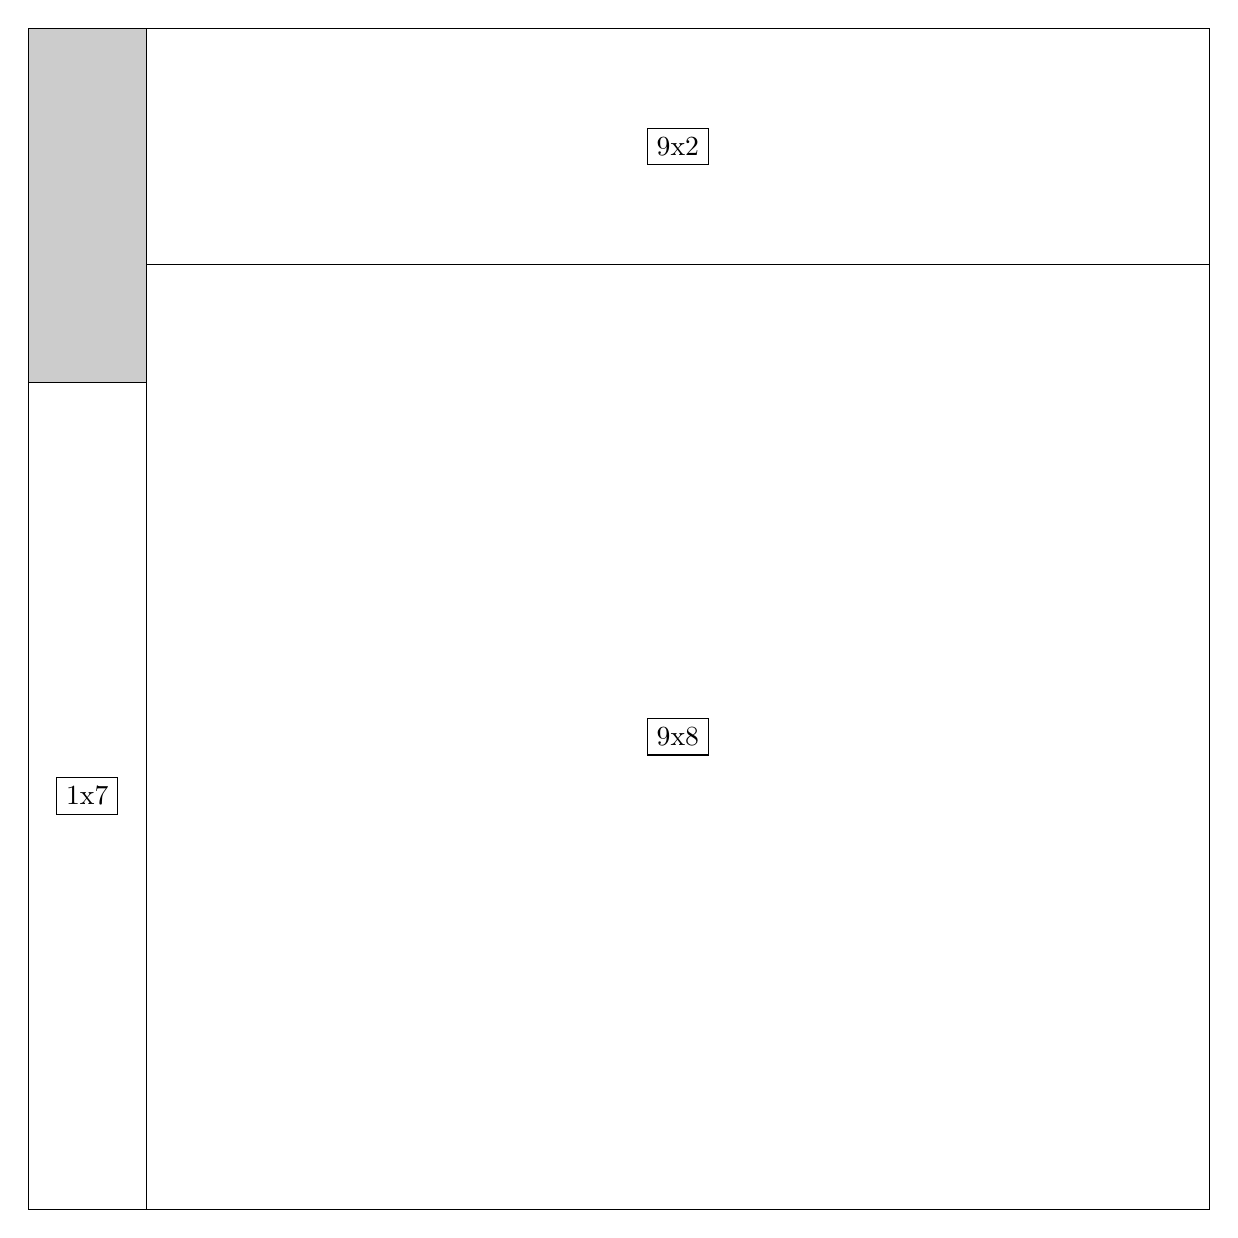
\begin{tikzpicture}[shorten >=1pt,scale=1.0,every node/.style={scale=1.0},->]
\tikzstyle{vertex}=[circle,fill=black!25,minimum size=14pt,inner sep=0pt]
\filldraw[fill=gray!40!white, draw=black] (0,0) rectangle (15.0,15.0);
\foreach \name/\x/\y/\w/\h in {9x8/1.5/0.0/13.5/12.0,1x7/0.0/0.0/1.5/10.5,9x2/1.5/12.0/13.5/3.0}
\filldraw[fill=white!40!white, draw=black] (\x,\y) rectangle node[draw] (\name) {\name} ++(\w,\h);
\end{tikzpicture}


w =9 , h =8 , x =1 , y =0 , v =72
\par
w =1 , h =7 , x =0 , y =0 , v =7
\par
w =9 , h =2 , x =1 , y =8 , v =18
\par
\newpage


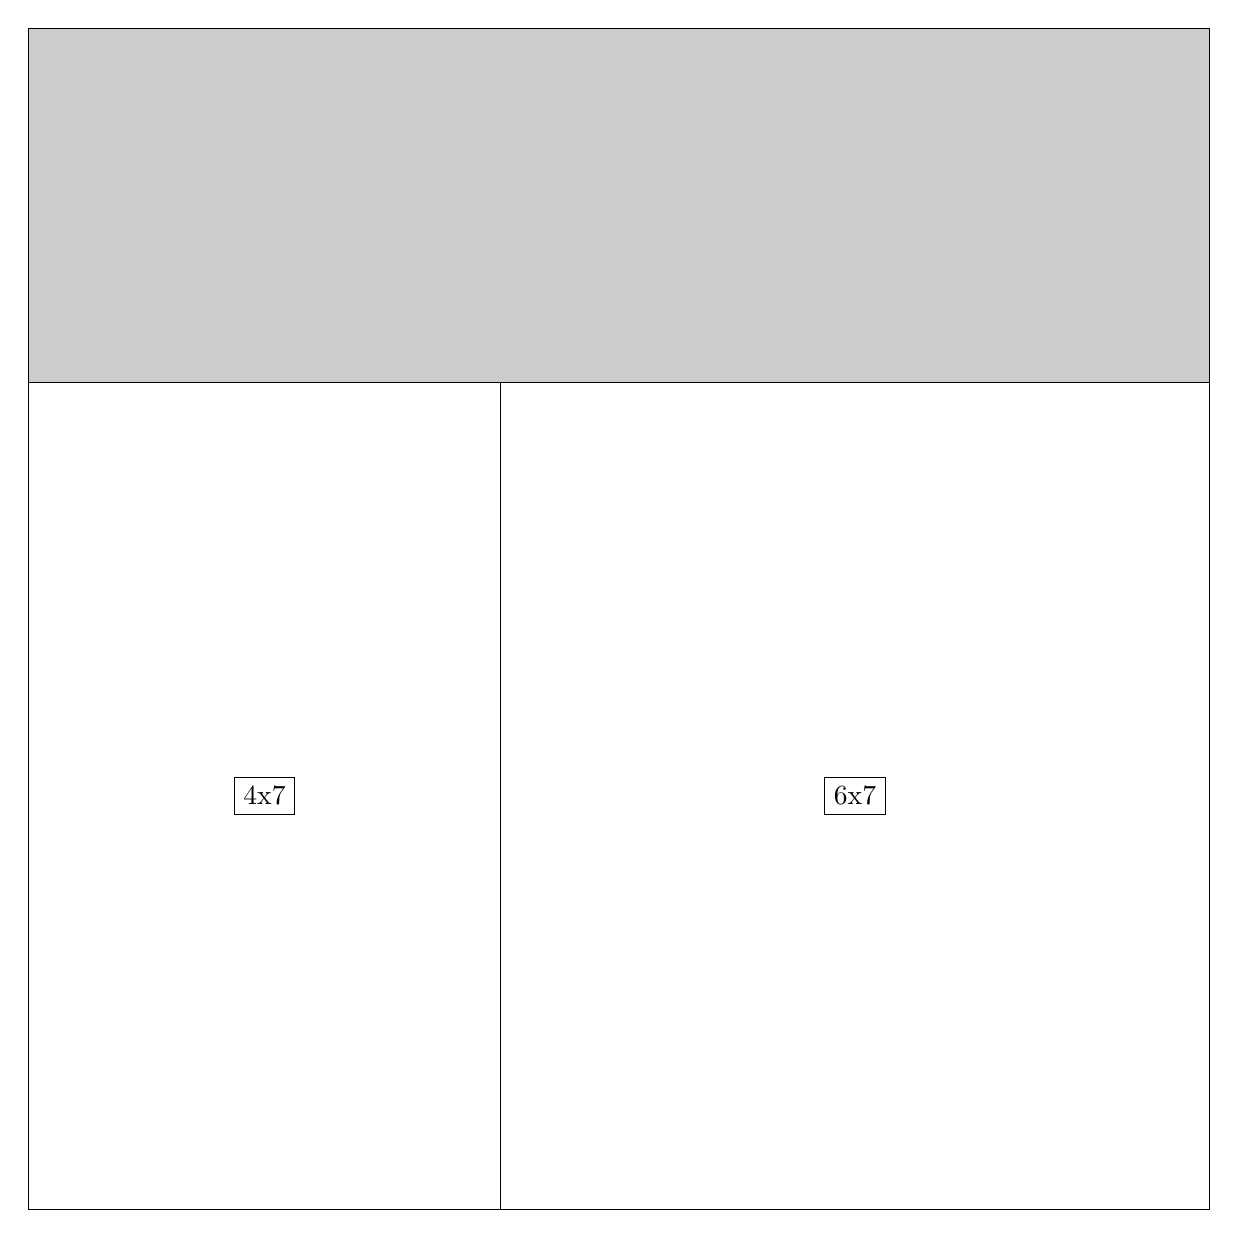
\begin{tikzpicture}[shorten >=1pt,scale=1.0,every node/.style={scale=1.0},->]
\tikzstyle{vertex}=[circle,fill=black!25,minimum size=14pt,inner sep=0pt]
\filldraw[fill=gray!40!white, draw=black] (0,0) rectangle (15.0,15.0);
\foreach \name/\x/\y/\w/\h in {6x7/6.0/0.0/9.0/10.5,4x7/0.0/0.0/6.0/10.5}
\filldraw[fill=white!40!white, draw=black] (\x,\y) rectangle node[draw] (\name) {\name} ++(\w,\h);
\end{tikzpicture}


w =6 , h =7 , x =4 , y =0 , v =42
\par
w =4 , h =7 , x =0 , y =0 , v =28
\par
\newpage


\begin{tikzpicture}[shorten >=1pt,scale=1.0,every node/.style={scale=1.0},->]
\tikzstyle{vertex}=[circle,fill=black!25,minimum size=14pt,inner sep=0pt]
\filldraw[fill=gray!40!white, draw=black] (0,0) rectangle (15.0,15.0);
\foreach \name/\x/\y/\w/\h in {7x7/4.5/0.0/10.5/10.5,3x7/0.0/0.0/4.5/10.5,10x3/0.0/10.5/15.0/4.5}
\filldraw[fill=white!40!white, draw=black] (\x,\y) rectangle node[draw] (\name) {\name} ++(\w,\h);
\end{tikzpicture}


w =7 , h =7 , x =3 , y =0 , v =49
\par
w =3 , h =7 , x =0 , y =0 , v =21
\par
w =10 , h =3 , x =0 , y =7 , v =30
\par
\newpage


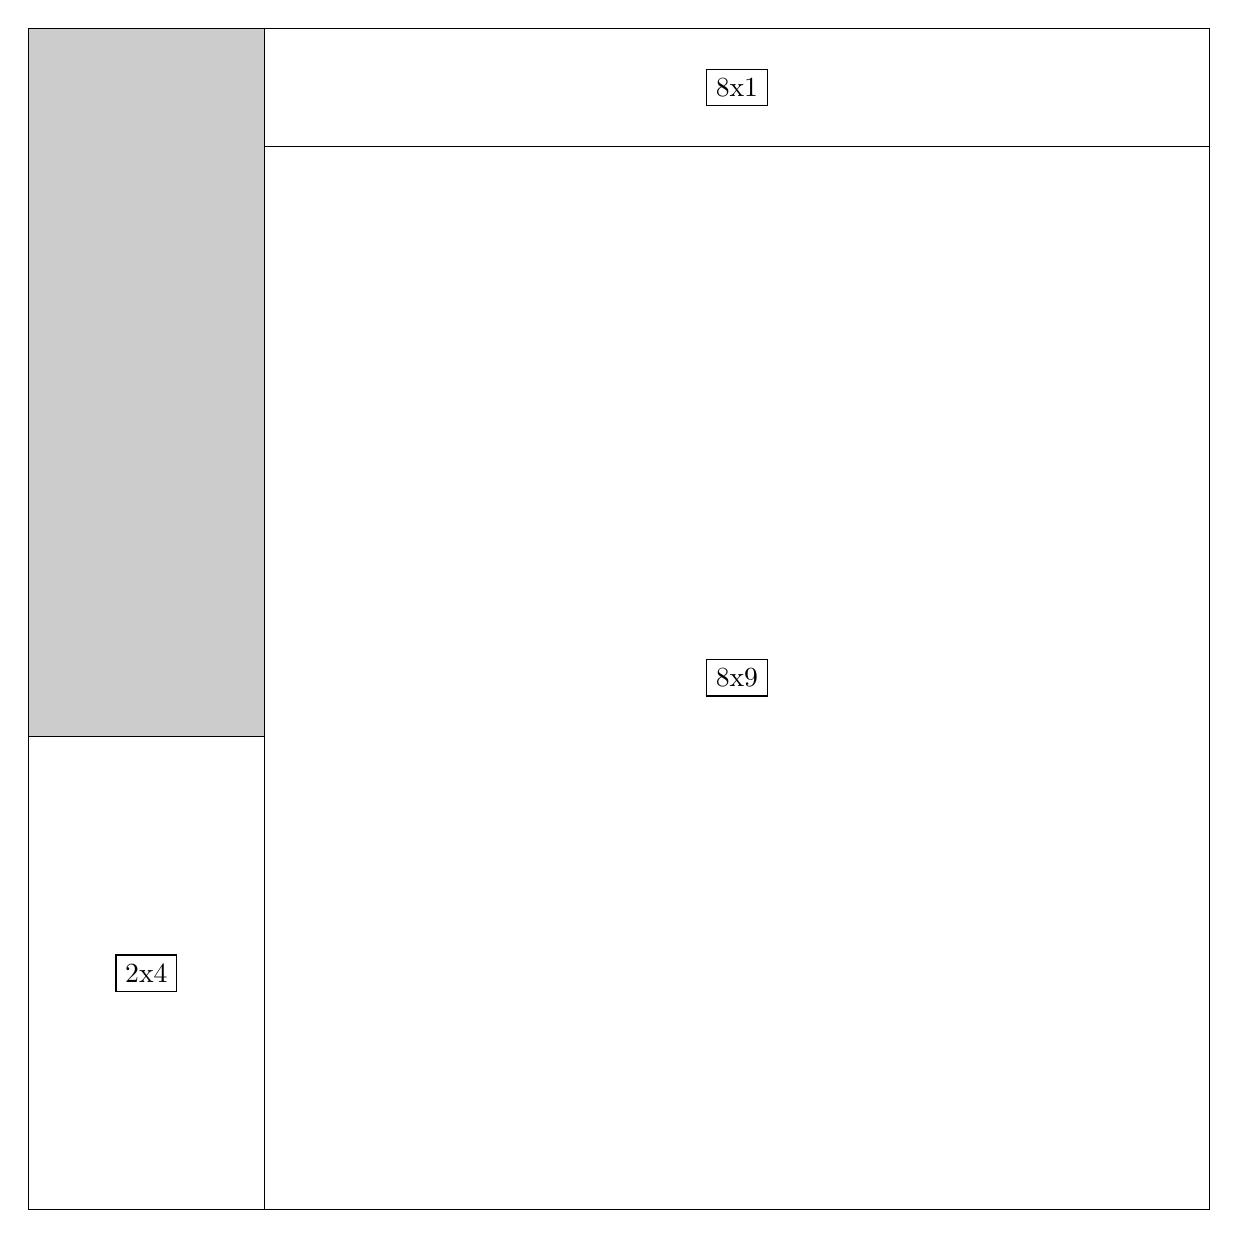
\begin{tikzpicture}[shorten >=1pt,scale=1.0,every node/.style={scale=1.0},->]
\tikzstyle{vertex}=[circle,fill=black!25,minimum size=14pt,inner sep=0pt]
\filldraw[fill=gray!40!white, draw=black] (0,0) rectangle (15.0,15.0);
\foreach \name/\x/\y/\w/\h in {8x9/3.0/0.0/12.0/13.5,8x1/3.0/13.5/12.0/1.5,2x4/0.0/0.0/3.0/6.0}
\filldraw[fill=white!40!white, draw=black] (\x,\y) rectangle node[draw] (\name) {\name} ++(\w,\h);
\end{tikzpicture}


w =8 , h =9 , x =2 , y =0 , v =72
\par
w =8 , h =1 , x =2 , y =9 , v =8
\par
w =2 , h =4 , x =0 , y =0 , v =8
\par
\newpage



\begin{tikzpicture}[shorten >=1pt,scale=1.0,every node/.style={scale=1.0},->]
\tikzstyle{vertex}=[circle,fill=black!25,minimum size=14pt,inner sep=0pt]
\filldraw[fill=gray!40!white, draw=black] (0,0) rectangle (15.0,15.0);
\foreach \name/\x/\y/\w/\h in {8x10/3.0/0.0/12.0/15.0}
\filldraw[fill=white!40!white, draw=black] (\x,\y) rectangle node[draw] (\name) {\name} ++(\w,\h);
\end{tikzpicture}


w =8 , h =10 , x =2 , y =0 , v =80
\par
\newpage


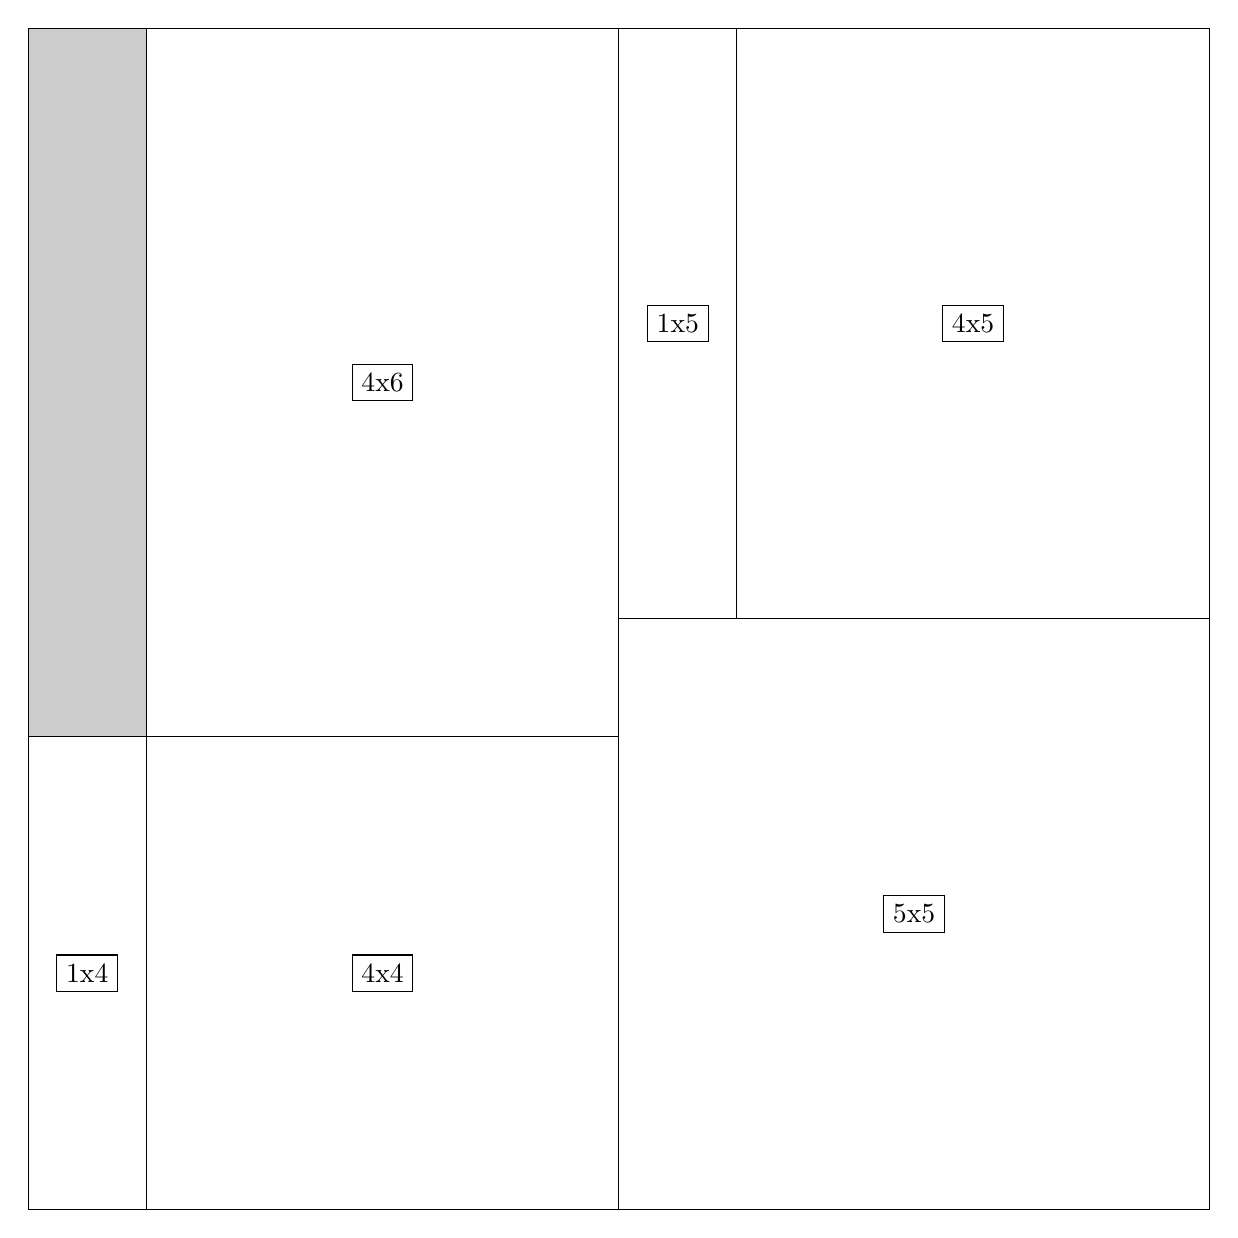
\begin{tikzpicture}[shorten >=1pt,scale=1.0,every node/.style={scale=1.0},->]
\tikzstyle{vertex}=[circle,fill=black!25,minimum size=14pt,inner sep=0pt]
\filldraw[fill=gray!40!white, draw=black] (0,0) rectangle (15.0,15.0);
\foreach \name/\x/\y/\w/\h in {5x5/7.5/0.0/7.5/7.5,4x5/9.0/7.5/6.0/7.5,1x5/7.5/7.5/1.5/7.5,4x4/1.5/0.0/6.0/6.0,1x4/0.0/0.0/1.5/6.0,4x6/1.5/6.0/6.0/9.0}
\filldraw[fill=white!40!white, draw=black] (\x,\y) rectangle node[draw] (\name) {\name} ++(\w,\h);
\end{tikzpicture}


w =5 , h =5 , x =5 , y =0 , v =25
\par
w =4 , h =5 , x =6 , y =5 , v =20
\par
w =1 , h =5 , x =5 , y =5 , v =5
\par
w =4 , h =4 , x =1 , y =0 , v =16
\par
w =1 , h =4 , x =0 , y =0 , v =4
\par
w =4 , h =6 , x =1 , y =4 , v =24
\par
\newpage


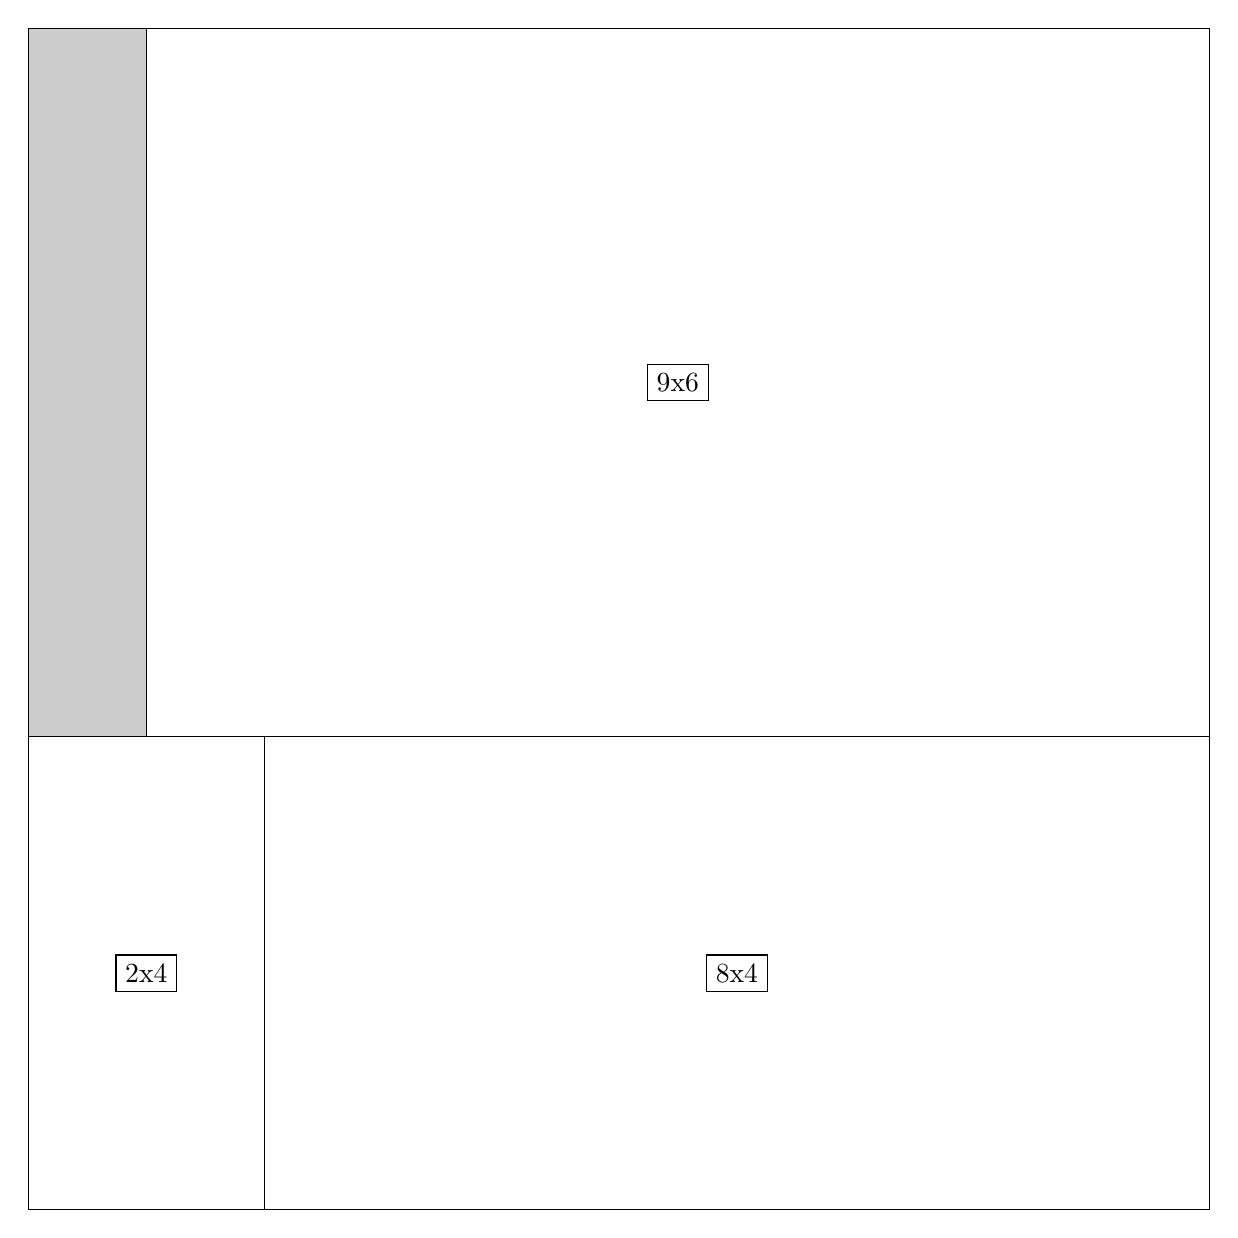
\begin{tikzpicture}[shorten >=1pt,scale=1.0,every node/.style={scale=1.0},->]
\tikzstyle{vertex}=[circle,fill=black!25,minimum size=14pt,inner sep=0pt]
\filldraw[fill=gray!40!white, draw=black] (0,0) rectangle (15.0,15.0);
\foreach \name/\x/\y/\w/\h in {8x4/3.0/0.0/12.0/6.0,2x4/0.0/0.0/3.0/6.0,9x6/1.5/6.0/13.5/9.0}
\filldraw[fill=white!40!white, draw=black] (\x,\y) rectangle node[draw] (\name) {\name} ++(\w,\h);
\end{tikzpicture}


w =8 , h =4 , x =2 , y =0 , v =32
\par
w =2 , h =4 , x =0 , y =0 , v =8
\par
w =9 , h =6 , x =1 , y =4 , v =54
\par
\newpage


\begin{tikzpicture}[shorten >=1pt,scale=1.0,every node/.style={scale=1.0},->]
\tikzstyle{vertex}=[circle,fill=black!25,minimum size=14pt,inner sep=0pt]
\filldraw[fill=gray!40!white, draw=black] (0,0) rectangle (15.0,15.0);
\foreach \name/\x/\y/\w/\h in {6x9/6.0/0.0/9.0/13.5,6x1/6.0/13.5/9.0/1.5,4x6/0.0/0.0/6.0/9.0,4x4/0.0/9.0/6.0/6.0}
\filldraw[fill=white!40!white, draw=black] (\x,\y) rectangle node[draw] (\name) {\name} ++(\w,\h);
\end{tikzpicture}


w =6 , h =9 , x =4 , y =0 , v =54
\par
w =6 , h =1 , x =4 , y =9 , v =6
\par
w =4 , h =6 , x =0 , y =0 , v =24
\par
w =4 , h =4 , x =0 , y =6 , v =16
\par
\newpage


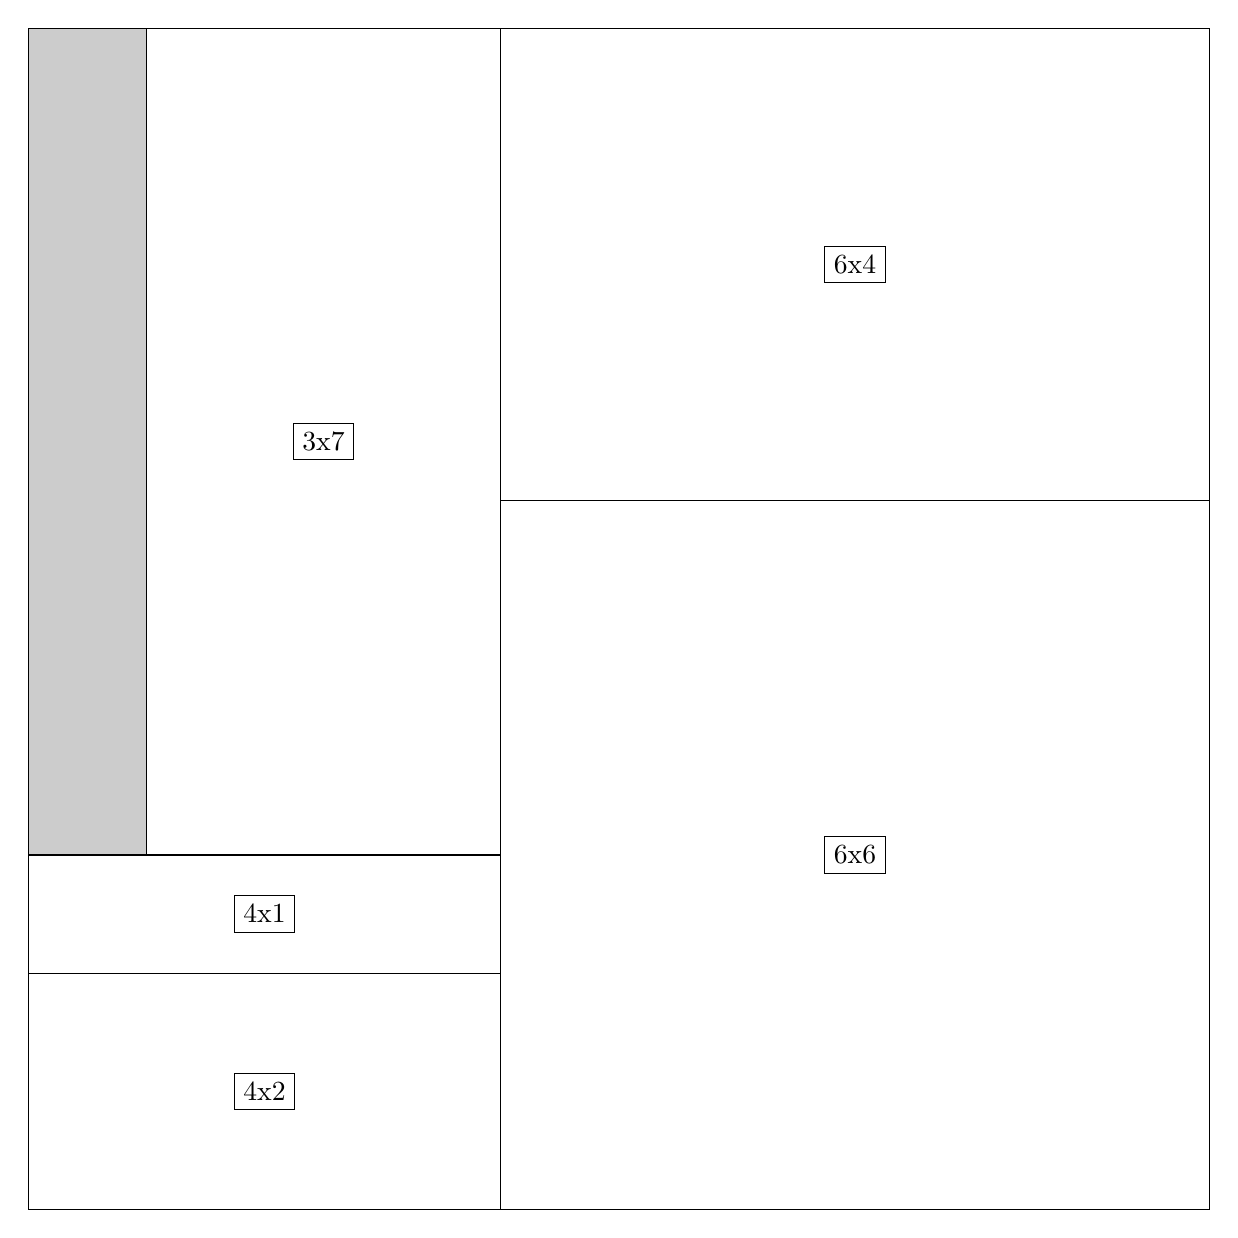
\begin{tikzpicture}[shorten >=1pt,scale=1.0,every node/.style={scale=1.0},->]
\tikzstyle{vertex}=[circle,fill=black!25,minimum size=14pt,inner sep=0pt]
\filldraw[fill=gray!40!white, draw=black] (0,0) rectangle (15.0,15.0);
\foreach \name/\x/\y/\w/\h in {6x6/6.0/0.0/9.0/9.0,6x4/6.0/9.0/9.0/6.0,4x2/0.0/0.0/6.0/3.0,4x1/0.0/3.0/6.0/1.5,3x7/1.5/4.5/4.5/10.5}
\filldraw[fill=white!40!white, draw=black] (\x,\y) rectangle node[draw] (\name) {\name} ++(\w,\h);
\end{tikzpicture}


w =6 , h =6 , x =4 , y =0 , v =36
\par
w =6 , h =4 , x =4 , y =6 , v =24
\par
w =4 , h =2 , x =0 , y =0 , v =8
\par
w =4 , h =1 , x =0 , y =2 , v =4
\par
w =3 , h =7 , x =1 , y =3 , v =21
\par
\newpage


\begin{tikzpicture}[shorten >=1pt,scale=1.0,every node/.style={scale=1.0},->]
\tikzstyle{vertex}=[circle,fill=black!25,minimum size=14pt,inner sep=0pt]
\filldraw[fill=gray!40!white, draw=black] (0,0) rectangle (15.0,15.0);
\foreach \name/\x/\y/\w/\h in {10x6/0.0/0.0/15.0/9.0,10x4/0.0/9.0/15.0/6.0}
\filldraw[fill=white!40!white, draw=black] (\x,\y) rectangle node[draw] (\name) {\name} ++(\w,\h);
\end{tikzpicture}


w =10 , h =6 , x =0 , y =0 , v =60
\par
w =10 , h =4 , x =0 , y =6 , v =40
\par
\newpage


\begin{tikzpicture}[shorten >=1pt,scale=1.0,every node/.style={scale=1.0},->]
\tikzstyle{vertex}=[circle,fill=black!25,minimum size=14pt,inner sep=0pt]
\filldraw[fill=gray!40!white, draw=black] (0,0) rectangle (15.0,15.0);
\foreach \name/\x/\y/\w/\h in {7x7/4.5/0.0/10.5/10.5,3x7/0.0/0.0/4.5/10.5,10x2/0.0/10.5/15.0/3.0,10x1/0.0/13.5/15.0/1.5}
\filldraw[fill=white!40!white, draw=black] (\x,\y) rectangle node[draw] (\name) {\name} ++(\w,\h);
\end{tikzpicture}


w =7 , h =7 , x =3 , y =0 , v =49
\par
w =3 , h =7 , x =0 , y =0 , v =21
\par
w =10 , h =2 , x =0 , y =7 , v =20
\par
w =10 , h =1 , x =0 , y =9 , v =10
\par
\newpage


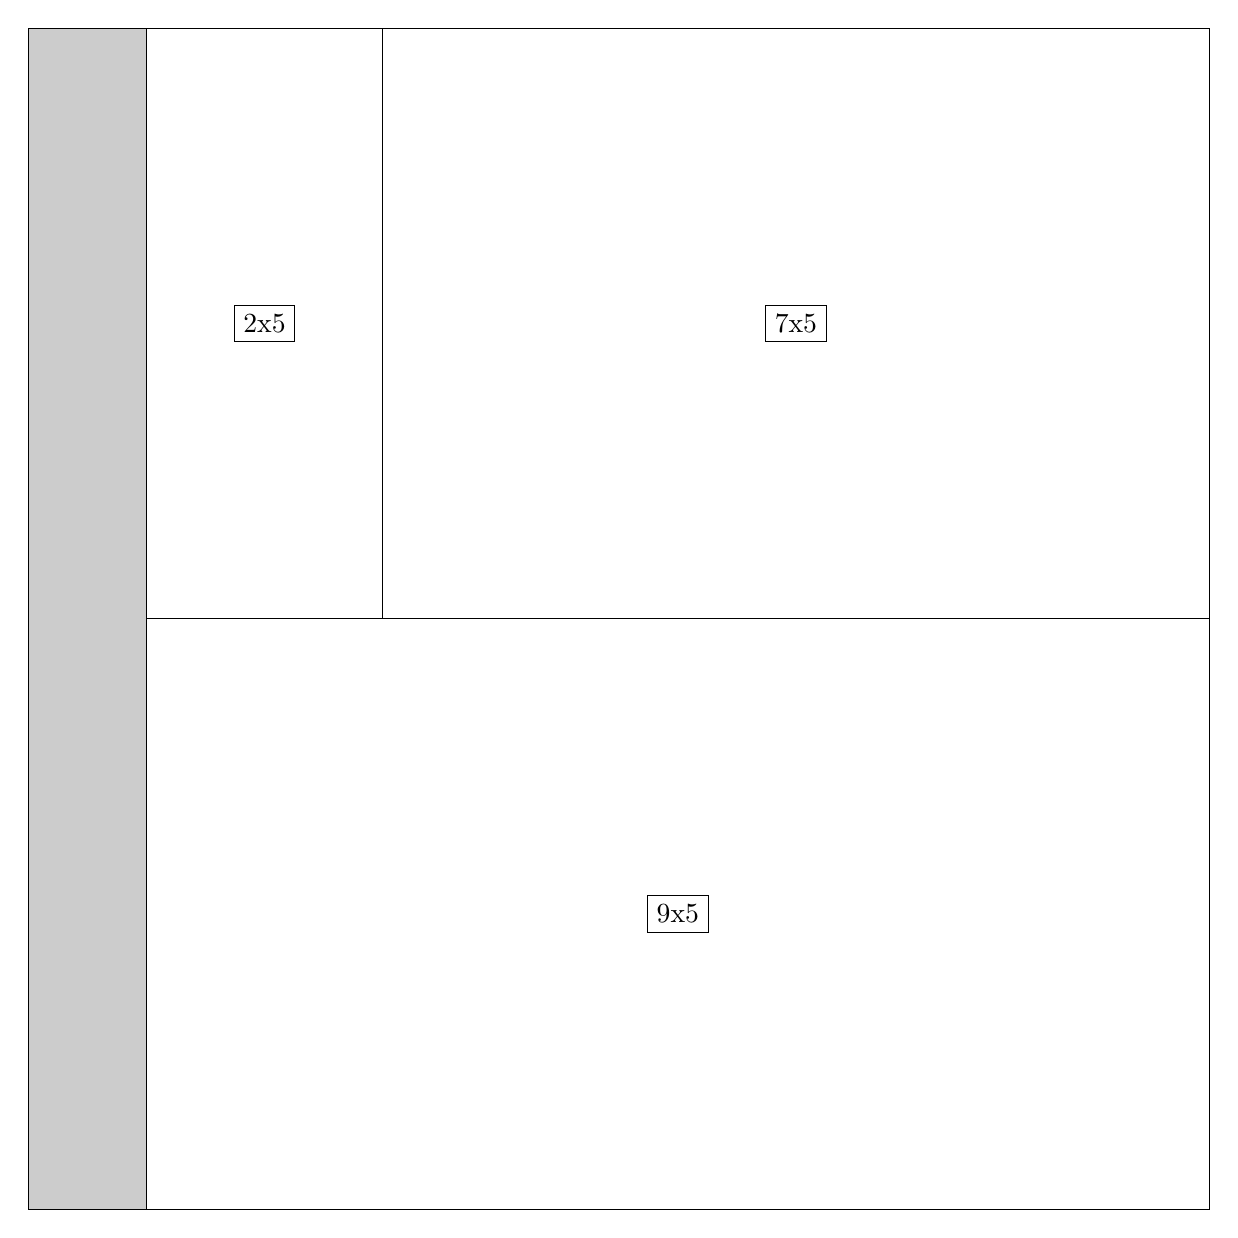
\begin{tikzpicture}[shorten >=1pt,scale=1.0,every node/.style={scale=1.0},->]
\tikzstyle{vertex}=[circle,fill=black!25,minimum size=14pt,inner sep=0pt]
\filldraw[fill=gray!40!white, draw=black] (0,0) rectangle (15.0,15.0);
\foreach \name/\x/\y/\w/\h in {9x5/1.5/0.0/13.5/7.5,7x5/4.5/7.5/10.5/7.5,2x5/1.5/7.5/3.0/7.5}
\filldraw[fill=white!40!white, draw=black] (\x,\y) rectangle node[draw] (\name) {\name} ++(\w,\h);
\end{tikzpicture}


w =9 , h =5 , x =1 , y =0 , v =45
\par
w =7 , h =5 , x =3 , y =5 , v =35
\par
w =2 , h =5 , x =1 , y =5 , v =10
\par
\newpage


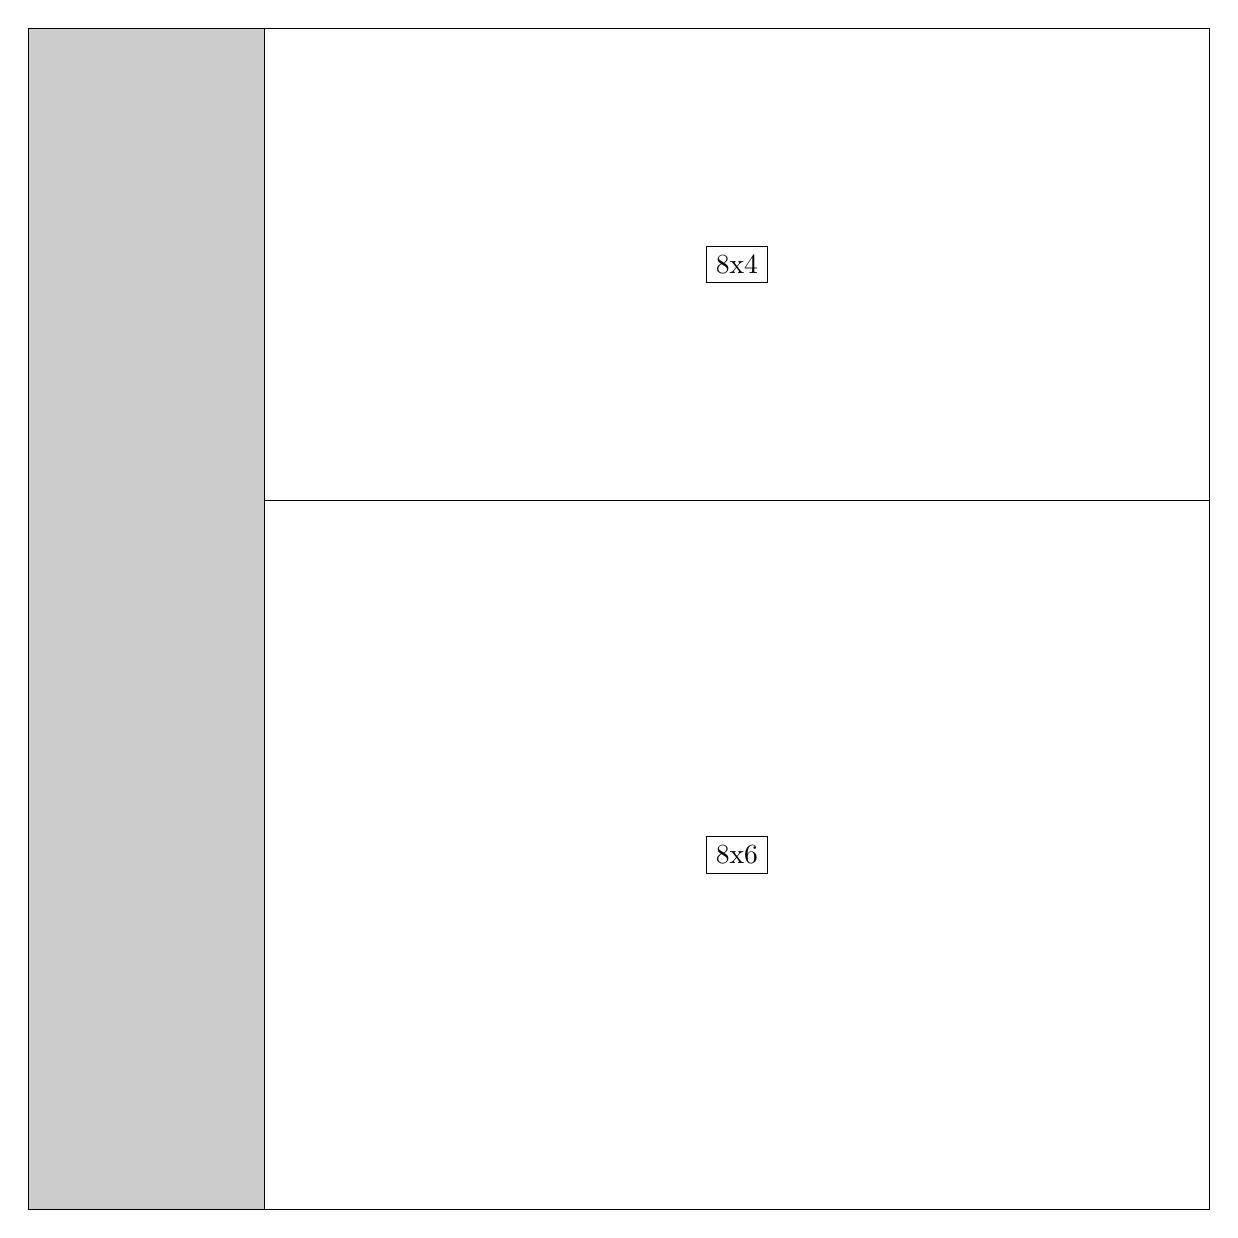
\begin{tikzpicture}[shorten >=1pt,scale=1.0,every node/.style={scale=1.0},->]
\tikzstyle{vertex}=[circle,fill=black!25,minimum size=14pt,inner sep=0pt]
\filldraw[fill=gray!40!white, draw=black] (0,0) rectangle (15.0,15.0);
\foreach \name/\x/\y/\w/\h in {8x6/3.0/0.0/12.0/9.0,8x4/3.0/9.0/12.0/6.0}
\filldraw[fill=white!40!white, draw=black] (\x,\y) rectangle node[draw] (\name) {\name} ++(\w,\h);
\end{tikzpicture}


w =8 , h =6 , x =2 , y =0 , v =48
\par
w =8 , h =4 , x =2 , y =6 , v =32
\par
\newpage


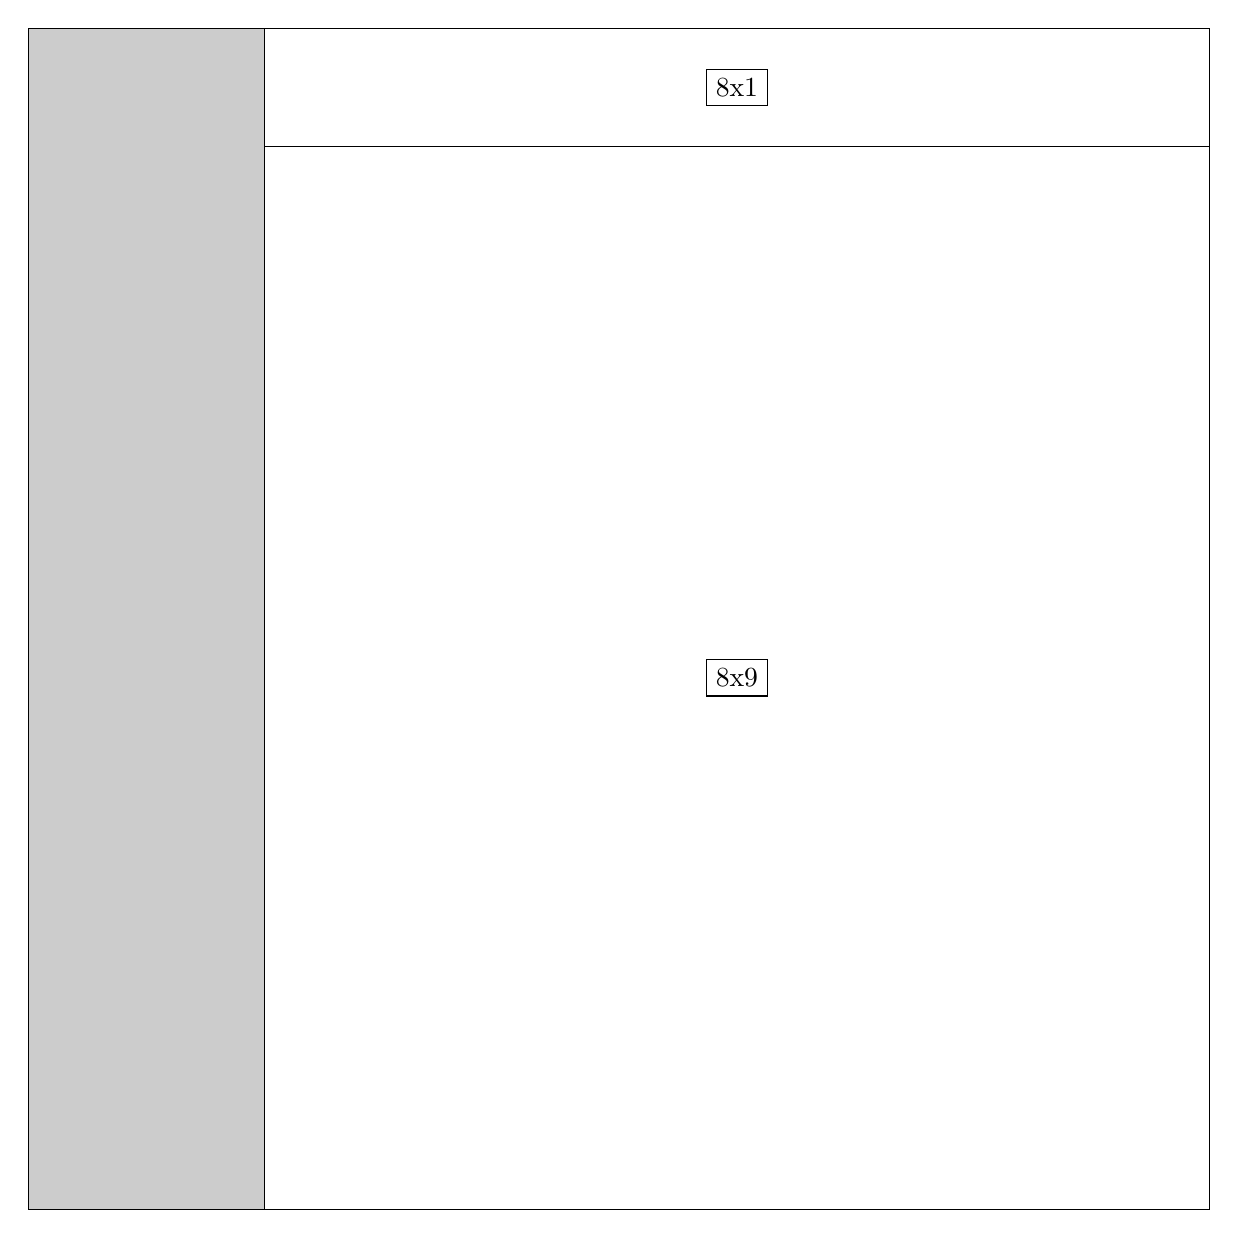
\begin{tikzpicture}[shorten >=1pt,scale=1.0,every node/.style={scale=1.0},->]
\tikzstyle{vertex}=[circle,fill=black!25,minimum size=14pt,inner sep=0pt]
\filldraw[fill=gray!40!white, draw=black] (0,0) rectangle (15.0,15.0);
\foreach \name/\x/\y/\w/\h in {8x9/3.0/0.0/12.0/13.5,8x1/3.0/13.5/12.0/1.5}
\filldraw[fill=white!40!white, draw=black] (\x,\y) rectangle node[draw] (\name) {\name} ++(\w,\h);
\end{tikzpicture}


w =8 , h =9 , x =2 , y =0 , v =72
\par
w =8 , h =1 , x =2 , y =9 , v =8
\par
\newpage


\begin{tikzpicture}[shorten >=1pt,scale=1.0,every node/.style={scale=1.0},->]
\tikzstyle{vertex}=[circle,fill=black!25,minimum size=14pt,inner sep=0pt]
\filldraw[fill=gray!40!white, draw=black] (0,0) rectangle (15.0,15.0);
\foreach \name/\x/\y/\w/\h in {7x7/4.5/0.0/10.5/10.5,7x3/4.5/10.5/10.5/4.5,3x8/0.0/0.0/4.5/12.0,3x2/0.0/12.0/4.5/3.0}
\filldraw[fill=white!40!white, draw=black] (\x,\y) rectangle node[draw] (\name) {\name} ++(\w,\h);
\end{tikzpicture}


w =7 , h =7 , x =3 , y =0 , v =49
\par
w =7 , h =3 , x =3 , y =7 , v =21
\par
w =3 , h =8 , x =0 , y =0 , v =24
\par
w =3 , h =2 , x =0 , y =8 , v =6
\par
\newpage


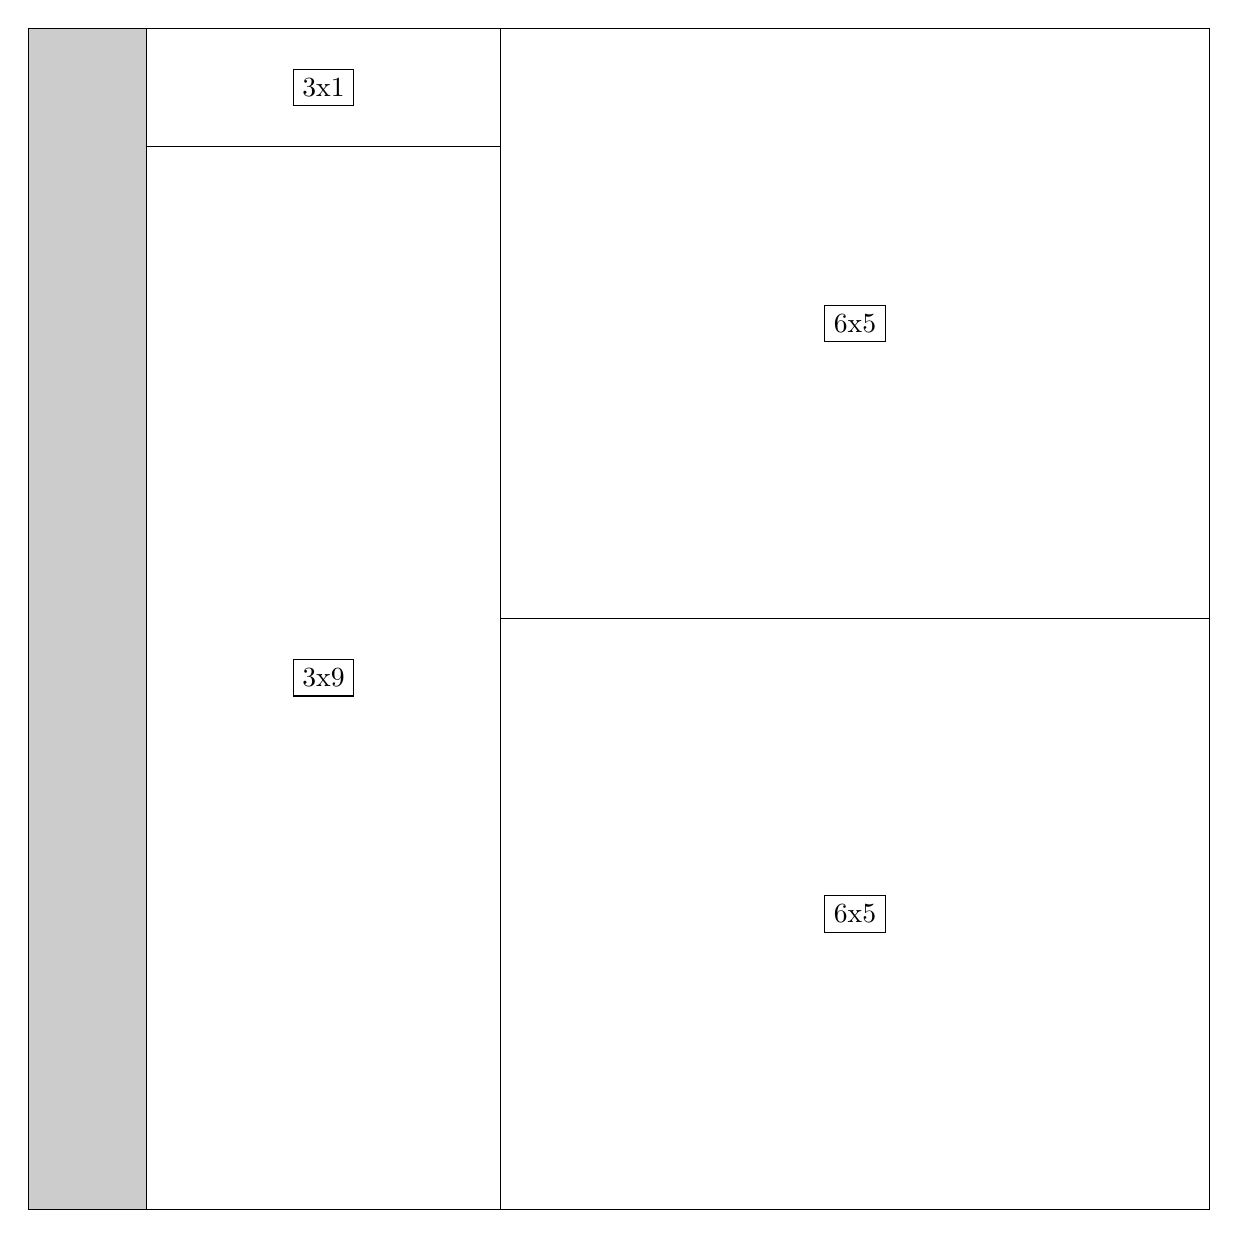
\begin{tikzpicture}[shorten >=1pt,scale=1.0,every node/.style={scale=1.0},->]
\tikzstyle{vertex}=[circle,fill=black!25,minimum size=14pt,inner sep=0pt]
\filldraw[fill=gray!40!white, draw=black] (0,0) rectangle (15.0,15.0);
\foreach \name/\x/\y/\w/\h in {6x5/6.0/0.0/9.0/7.5,6x5/6.0/7.5/9.0/7.5,3x9/1.5/0.0/4.5/13.5,3x1/1.5/13.5/4.5/1.5}
\filldraw[fill=white!40!white, draw=black] (\x,\y) rectangle node[draw] (\name) {\name} ++(\w,\h);
\end{tikzpicture}


w =6 , h =5 , x =4 , y =0 , v =30
\par
w =6 , h =5 , x =4 , y =5 , v =30
\par
w =3 , h =9 , x =1 , y =0 , v =27
\par
w =3 , h =1 , x =1 , y =9 , v =3
\par
\newpage


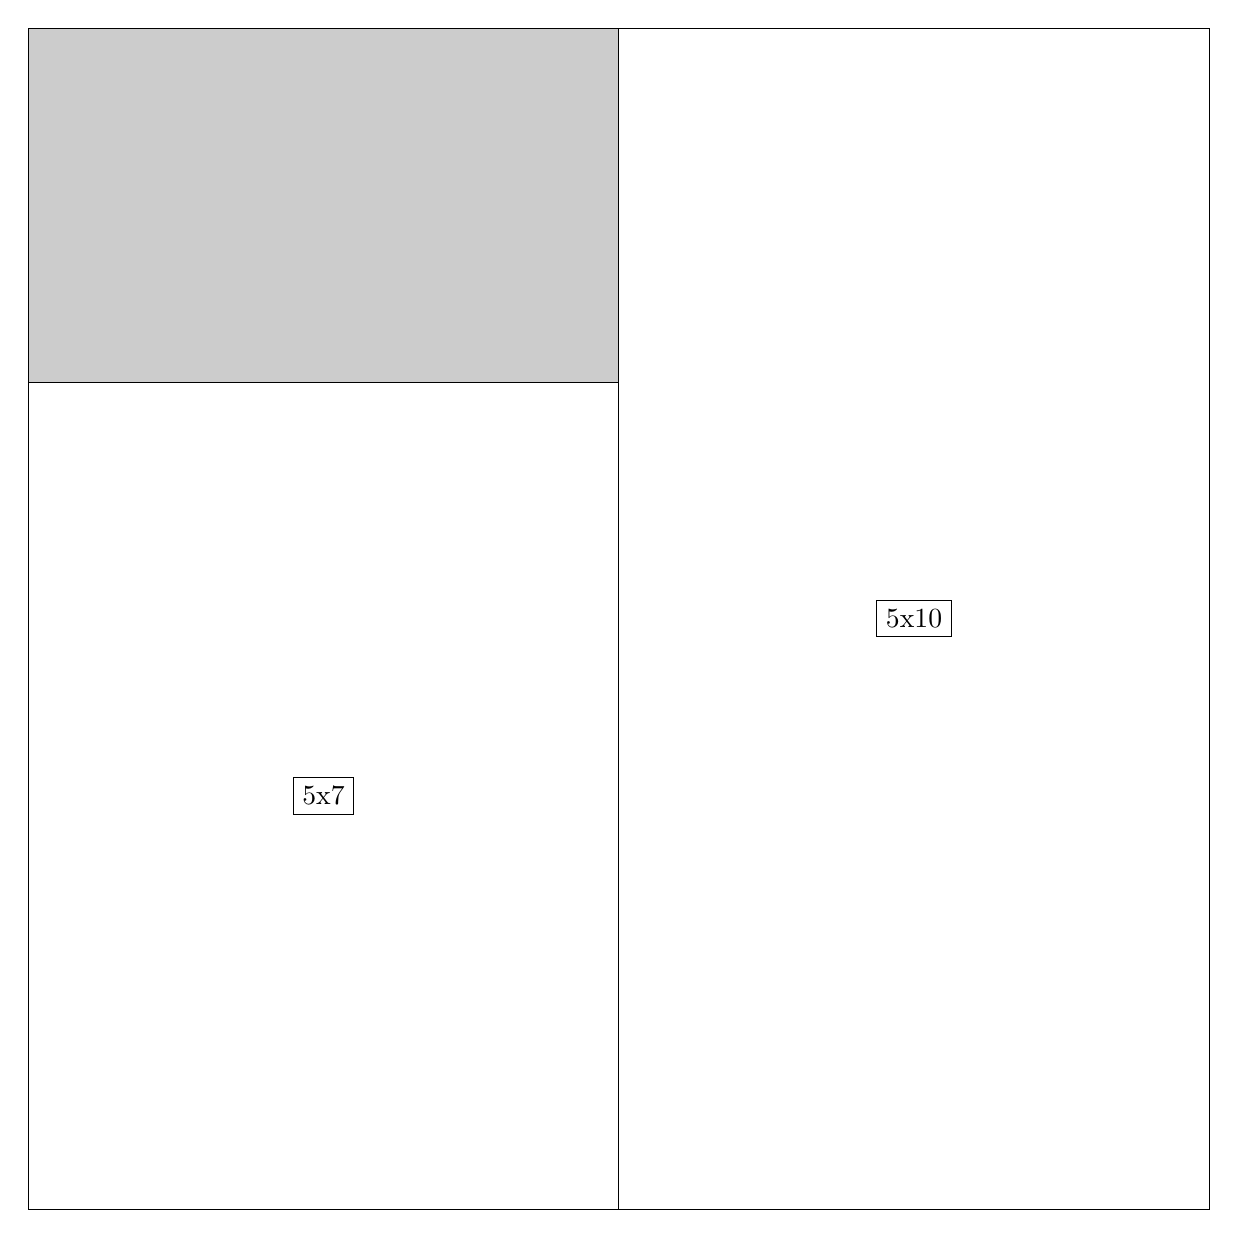
\begin{tikzpicture}[shorten >=1pt,scale=1.0,every node/.style={scale=1.0},->]
\tikzstyle{vertex}=[circle,fill=black!25,minimum size=14pt,inner sep=0pt]
\filldraw[fill=gray!40!white, draw=black] (0,0) rectangle (15.0,15.0);
\foreach \name/\x/\y/\w/\h in {5x10/7.5/0.0/7.5/15.0,5x7/0.0/0.0/7.5/10.5}
\filldraw[fill=white!40!white, draw=black] (\x,\y) rectangle node[draw] (\name) {\name} ++(\w,\h);
\end{tikzpicture}


w =5 , h =10 , x =5 , y =0 , v =50
\par
w =5 , h =7 , x =0 , y =0 , v =35
\par
\newpage


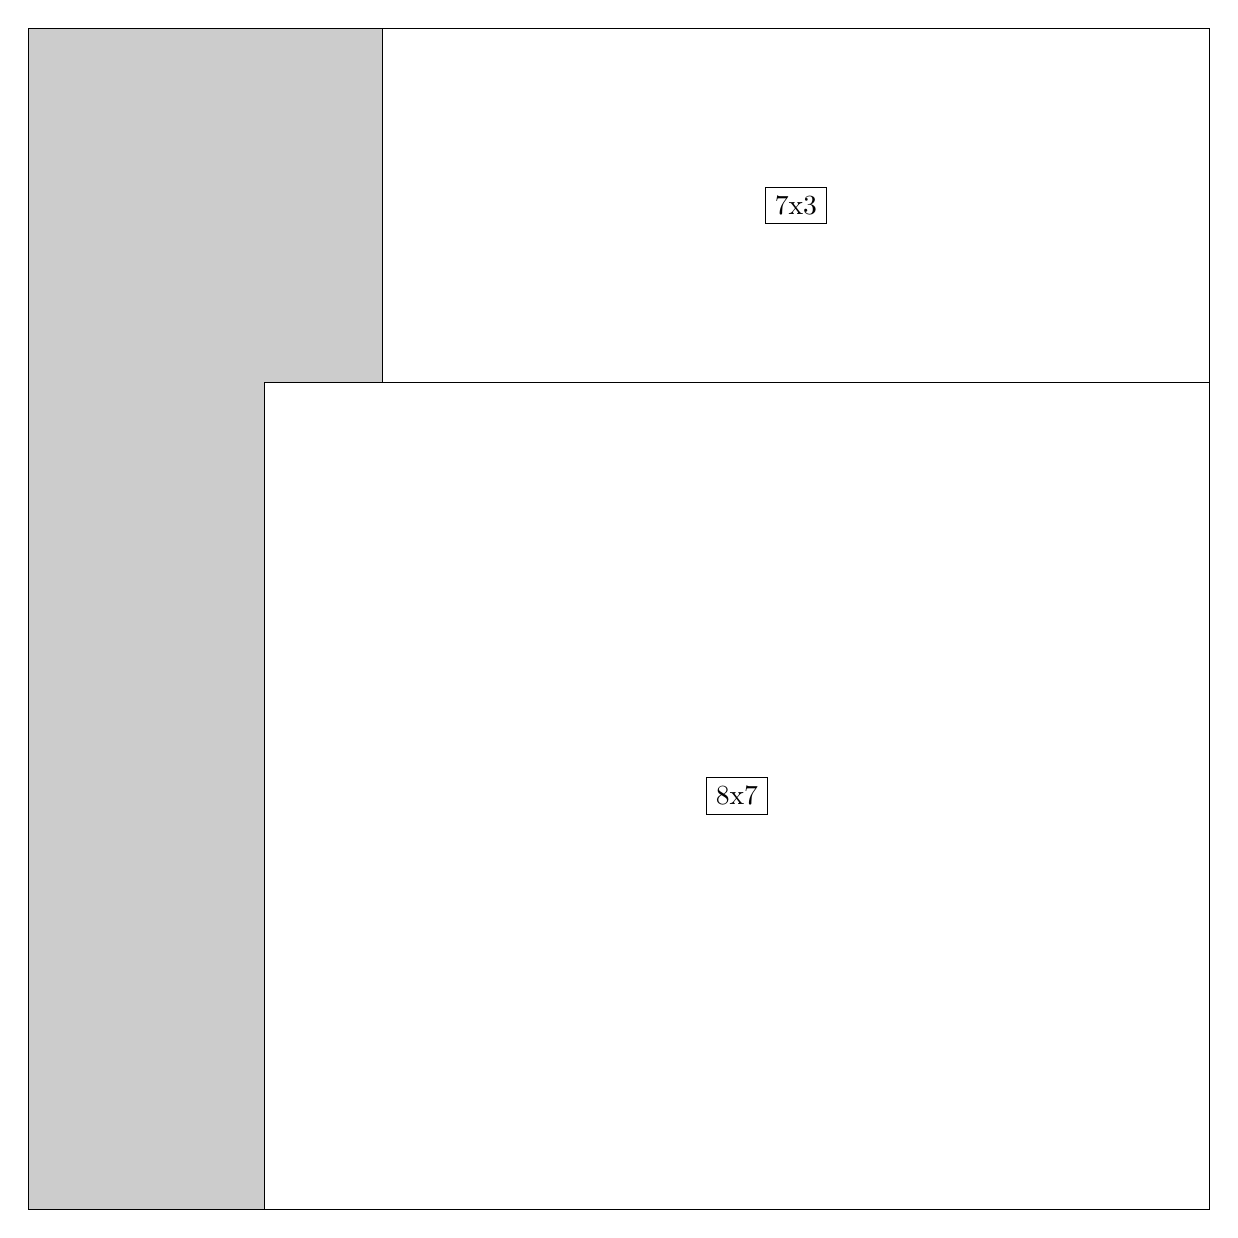
\begin{tikzpicture}[shorten >=1pt,scale=1.0,every node/.style={scale=1.0},->]
\tikzstyle{vertex}=[circle,fill=black!25,minimum size=14pt,inner sep=0pt]
\filldraw[fill=gray!40!white, draw=black] (0,0) rectangle (15.0,15.0);
\foreach \name/\x/\y/\w/\h in {8x7/3.0/0.0/12.0/10.5,7x3/4.5/10.5/10.5/4.5}
\filldraw[fill=white!40!white, draw=black] (\x,\y) rectangle node[draw] (\name) {\name} ++(\w,\h);
\end{tikzpicture}


w =8 , h =7 , x =2 , y =0 , v =56
\par
w =7 , h =3 , x =3 , y =7 , v =21
\par
\newpage


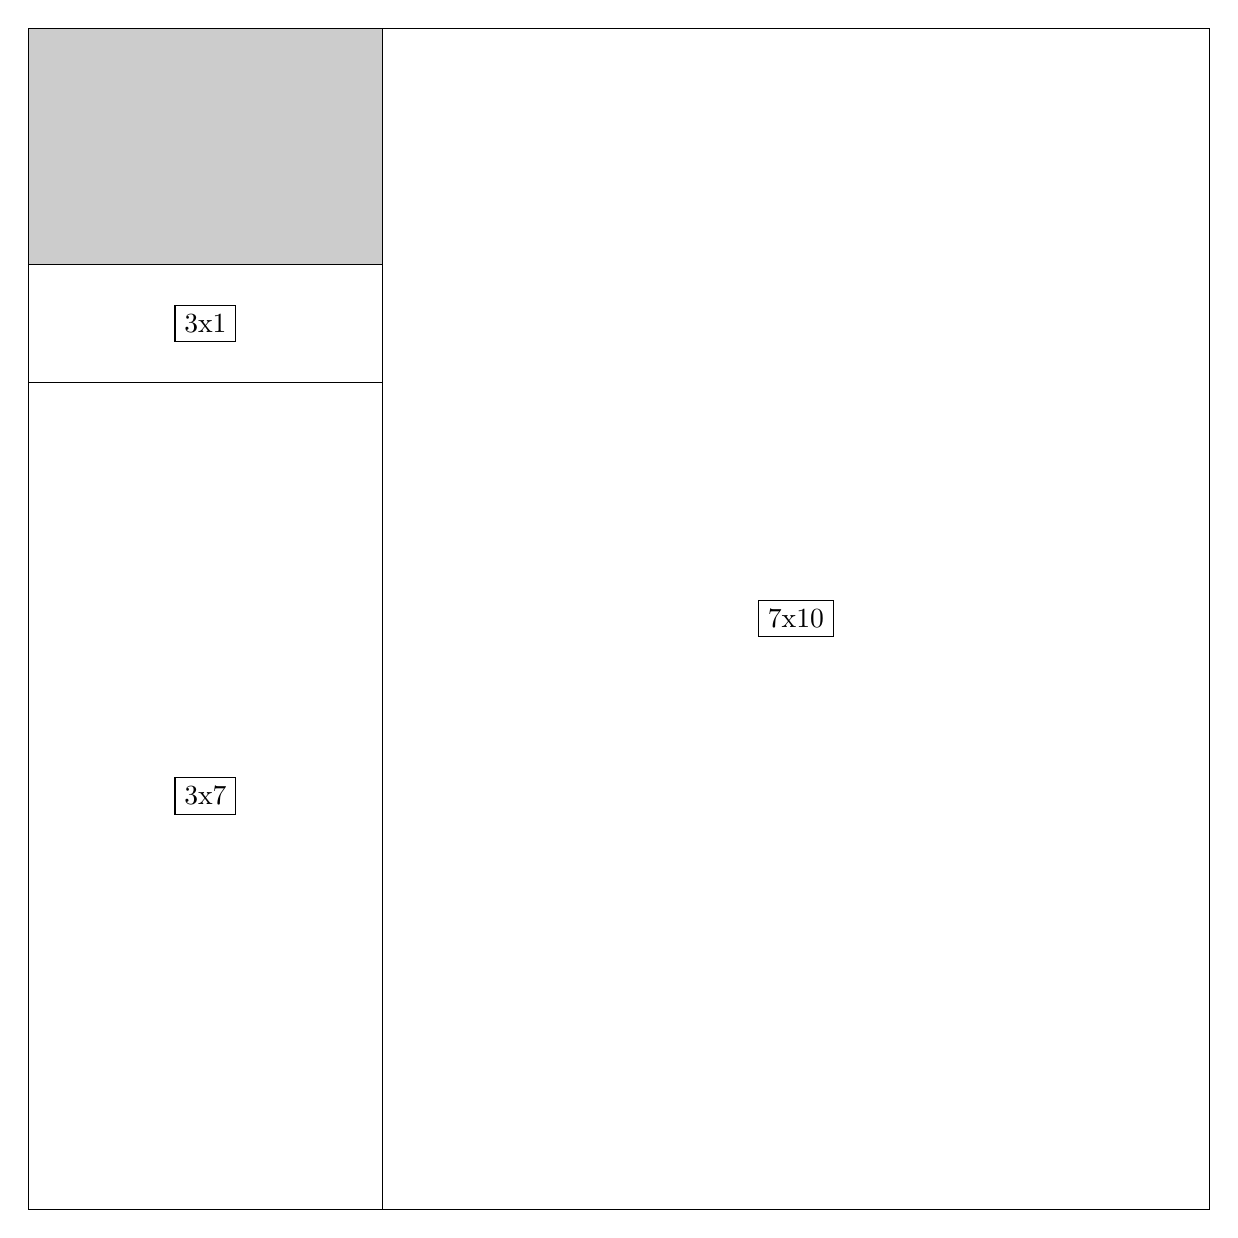
\begin{tikzpicture}[shorten >=1pt,scale=1.0,every node/.style={scale=1.0},->]
\tikzstyle{vertex}=[circle,fill=black!25,minimum size=14pt,inner sep=0pt]
\filldraw[fill=gray!40!white, draw=black] (0,0) rectangle (15.0,15.0);
\foreach \name/\x/\y/\w/\h in {7x10/4.5/0.0/10.5/15.0,3x7/0.0/0.0/4.5/10.5,3x1/0.0/10.5/4.5/1.5}
\filldraw[fill=white!40!white, draw=black] (\x,\y) rectangle node[draw] (\name) {\name} ++(\w,\h);
\end{tikzpicture}


w =7 , h =10 , x =3 , y =0 , v =70
\par
w =3 , h =7 , x =0 , y =0 , v =21
\par
w =3 , h =1 , x =0 , y =7 , v =3
\par
\newpage



\begin{tikzpicture}[shorten >=1pt,scale=1.0,every node/.style={scale=1.0},->]
\tikzstyle{vertex}=[circle,fill=black!25,minimum size=14pt,inner sep=0pt]
\filldraw[fill=gray!40!white, draw=black] (0,0) rectangle (15.0,15.0);
\foreach \name/\x/\y/\w/\h in {8x10/3.0/0.0/12.0/15.0}
\filldraw[fill=white!40!white, draw=black] (\x,\y) rectangle node[draw] (\name) {\name} ++(\w,\h);
\end{tikzpicture}


w =8 , h =10 , x =2 , y =0 , v =80
\par
\newpage


\begin{tikzpicture}[shorten >=1pt,scale=1.0,every node/.style={scale=1.0},->]
\tikzstyle{vertex}=[circle,fill=black!25,minimum size=14pt,inner sep=0pt]
\filldraw[fill=gray!40!white, draw=black] (0,0) rectangle (15.0,15.0);
\foreach \name/\x/\y/\w/\h in {10x8/0.0/0.0/15.0/12.0,10x2/0.0/12.0/15.0/3.0}
\filldraw[fill=white!40!white, draw=black] (\x,\y) rectangle node[draw] (\name) {\name} ++(\w,\h);
\end{tikzpicture}


w =10 , h =8 , x =0 , y =0 , v =80
\par
w =10 , h =2 , x =0 , y =8 , v =20
\par
\newpage


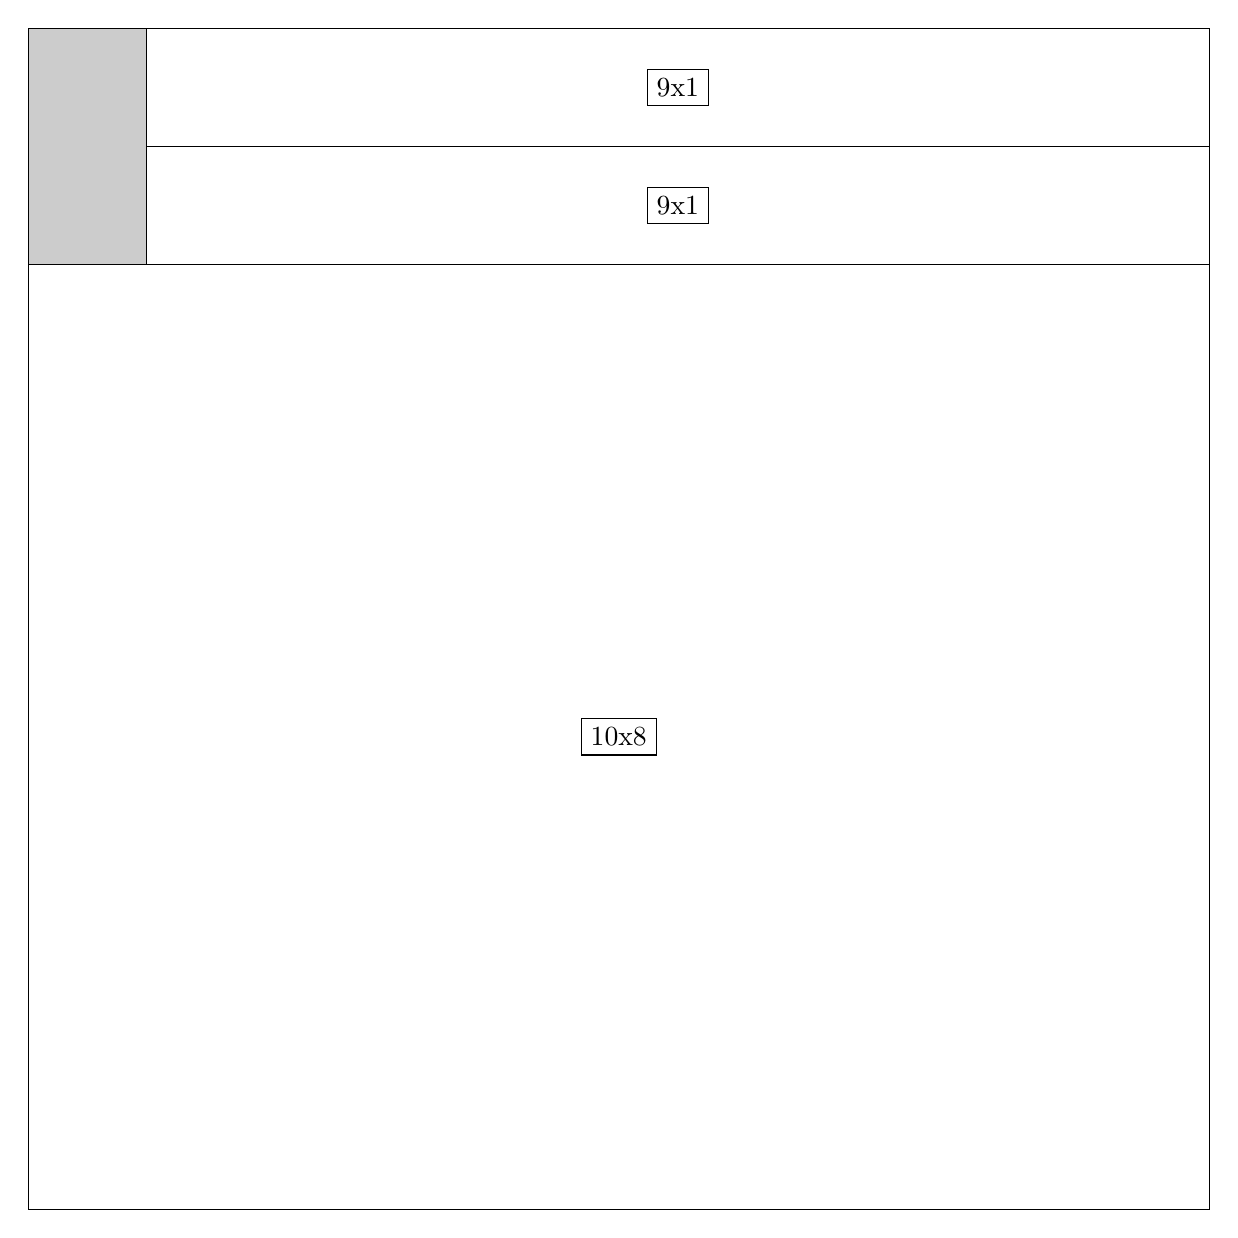
\begin{tikzpicture}[shorten >=1pt,scale=1.0,every node/.style={scale=1.0},->]
\tikzstyle{vertex}=[circle,fill=black!25,minimum size=14pt,inner sep=0pt]
\filldraw[fill=gray!40!white, draw=black] (0,0) rectangle (15.0,15.0);
\foreach \name/\x/\y/\w/\h in {10x8/0.0/0.0/15.0/12.0,9x1/1.5/12.0/13.5/1.5,9x1/1.5/13.5/13.5/1.5}
\filldraw[fill=white!40!white, draw=black] (\x,\y) rectangle node[draw] (\name) {\name} ++(\w,\h);
\end{tikzpicture}


w =10 , h =8 , x =0 , y =0 , v =80
\par
w =9 , h =1 , x =1 , y =8 , v =9
\par
w =9 , h =1 , x =1 , y =9 , v =9
\par
\newpage


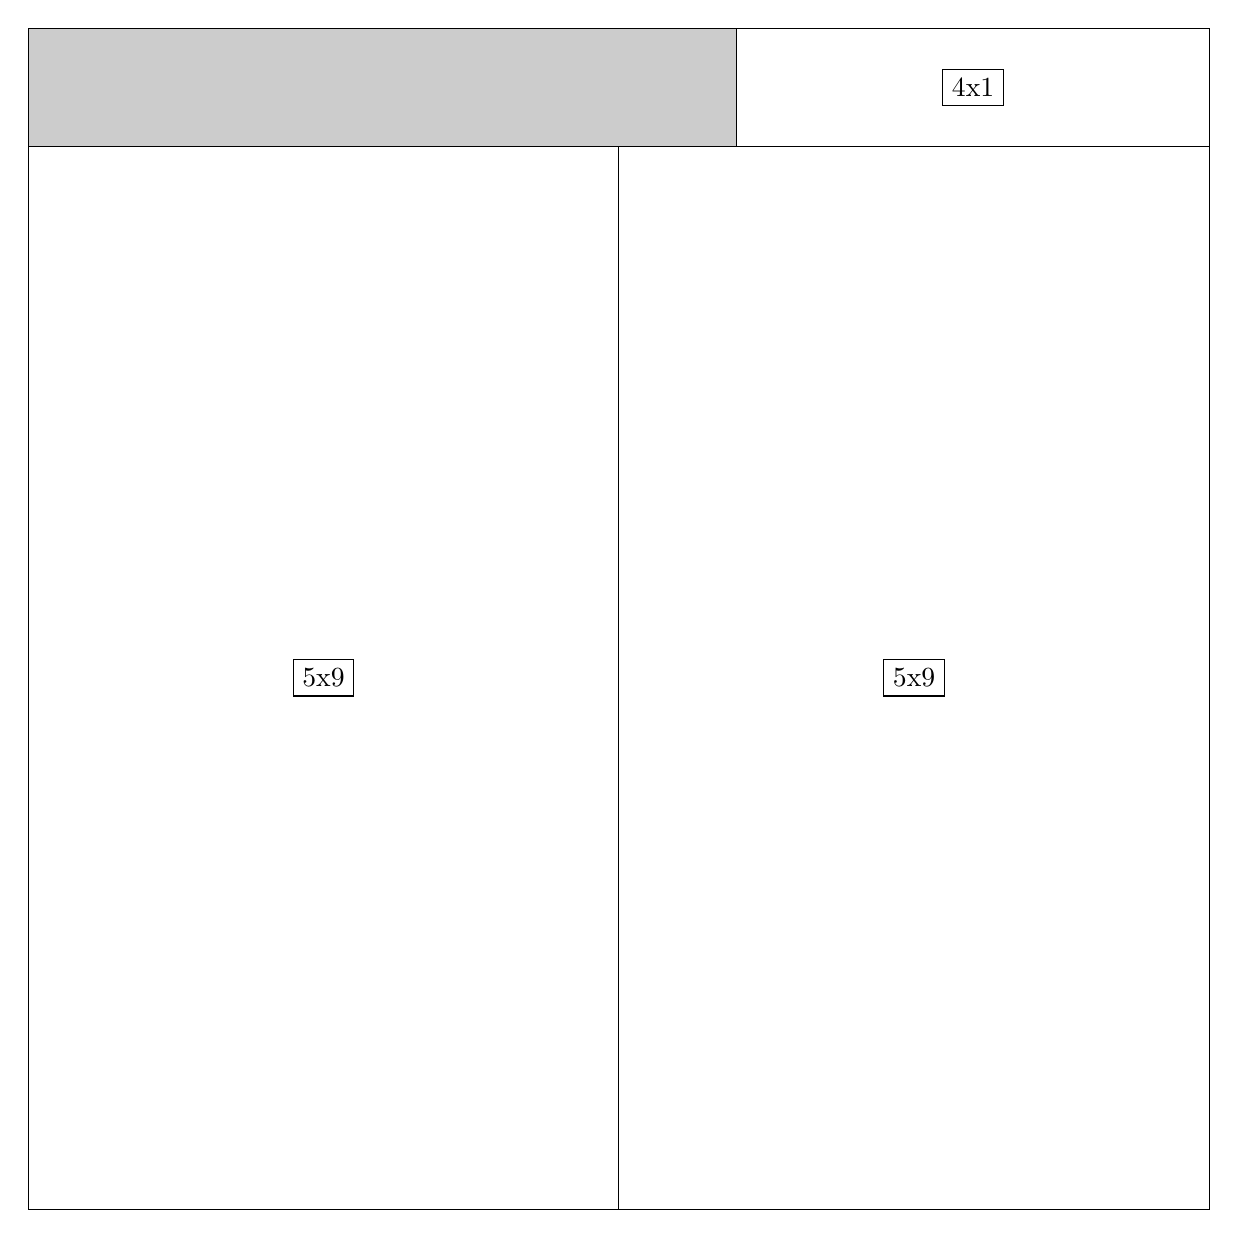
\begin{tikzpicture}[shorten >=1pt,scale=1.0,every node/.style={scale=1.0},->]
\tikzstyle{vertex}=[circle,fill=black!25,minimum size=14pt,inner sep=0pt]
\filldraw[fill=gray!40!white, draw=black] (0,0) rectangle (15.0,15.0);
\foreach \name/\x/\y/\w/\h in {5x9/7.5/0.0/7.5/13.5,4x1/9.0/13.5/6.0/1.5,5x9/0.0/0.0/7.5/13.5}
\filldraw[fill=white!40!white, draw=black] (\x,\y) rectangle node[draw] (\name) {\name} ++(\w,\h);
\end{tikzpicture}


w =5 , h =9 , x =5 , y =0 , v =45
\par
w =4 , h =1 , x =6 , y =9 , v =4
\par
w =5 , h =9 , x =0 , y =0 , v =45
\par
\newpage


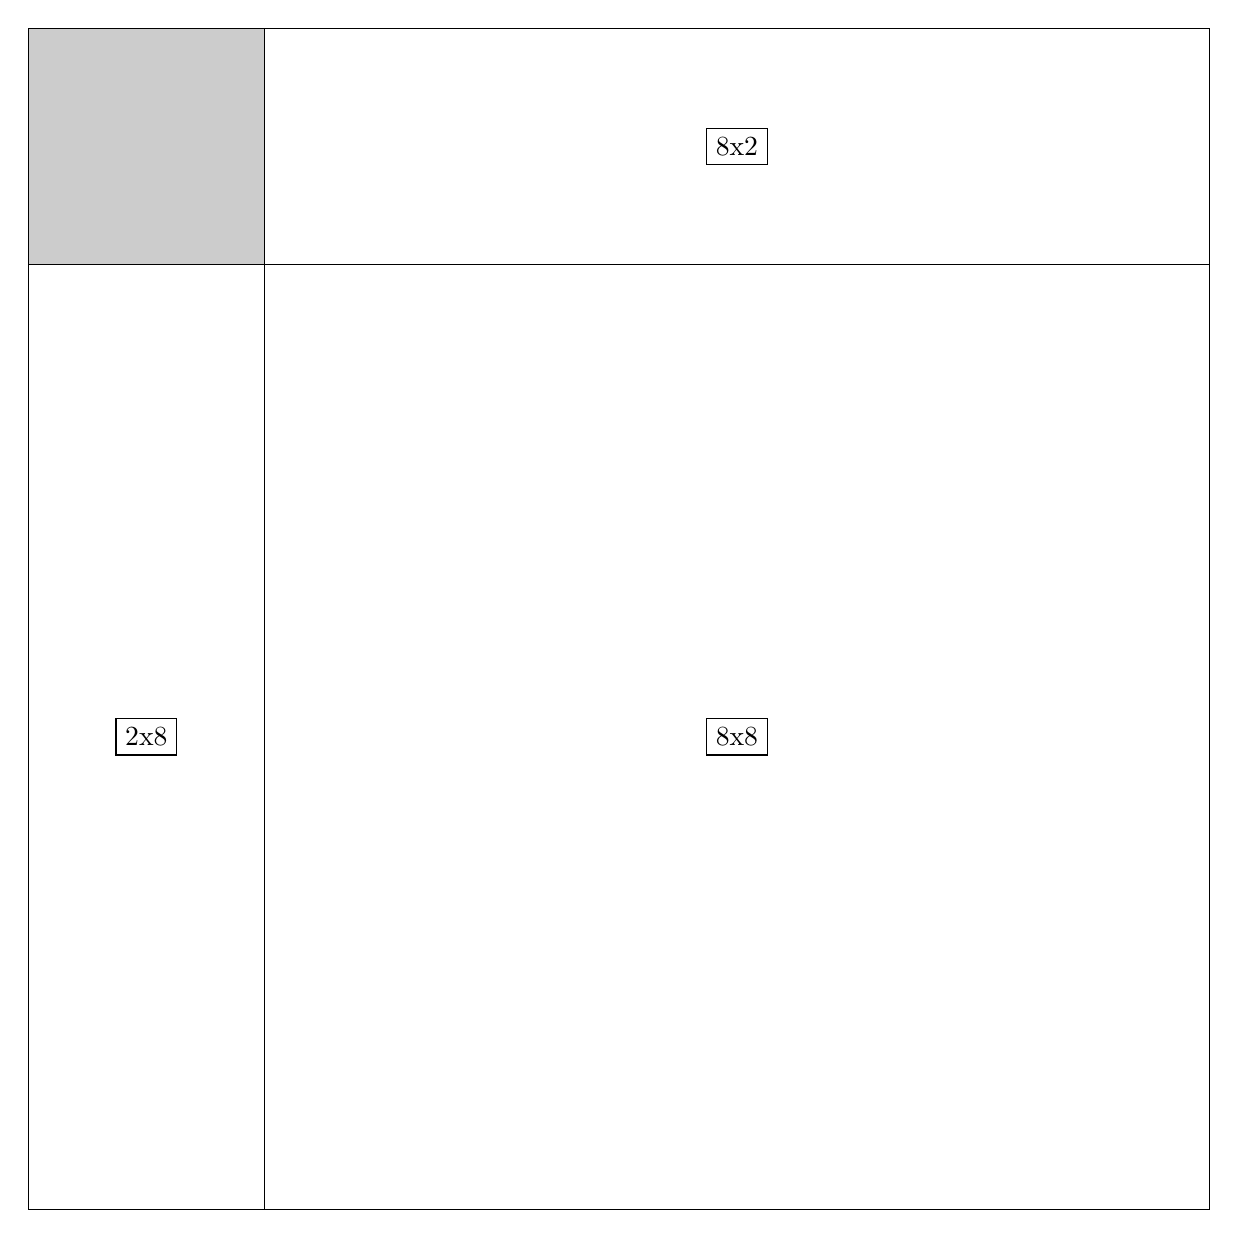
\begin{tikzpicture}[shorten >=1pt,scale=1.0,every node/.style={scale=1.0},->]
\tikzstyle{vertex}=[circle,fill=black!25,minimum size=14pt,inner sep=0pt]
\filldraw[fill=gray!40!white, draw=black] (0,0) rectangle (15.0,15.0);
\foreach \name/\x/\y/\w/\h in {8x8/3.0/0.0/12.0/12.0,8x2/3.0/12.0/12.0/3.0,2x8/0.0/0.0/3.0/12.0}
\filldraw[fill=white!40!white, draw=black] (\x,\y) rectangle node[draw] (\name) {\name} ++(\w,\h);
\end{tikzpicture}


w =8 , h =8 , x =2 , y =0 , v =64
\par
w =8 , h =2 , x =2 , y =8 , v =16
\par
w =2 , h =8 , x =0 , y =0 , v =16
\par
\newpage


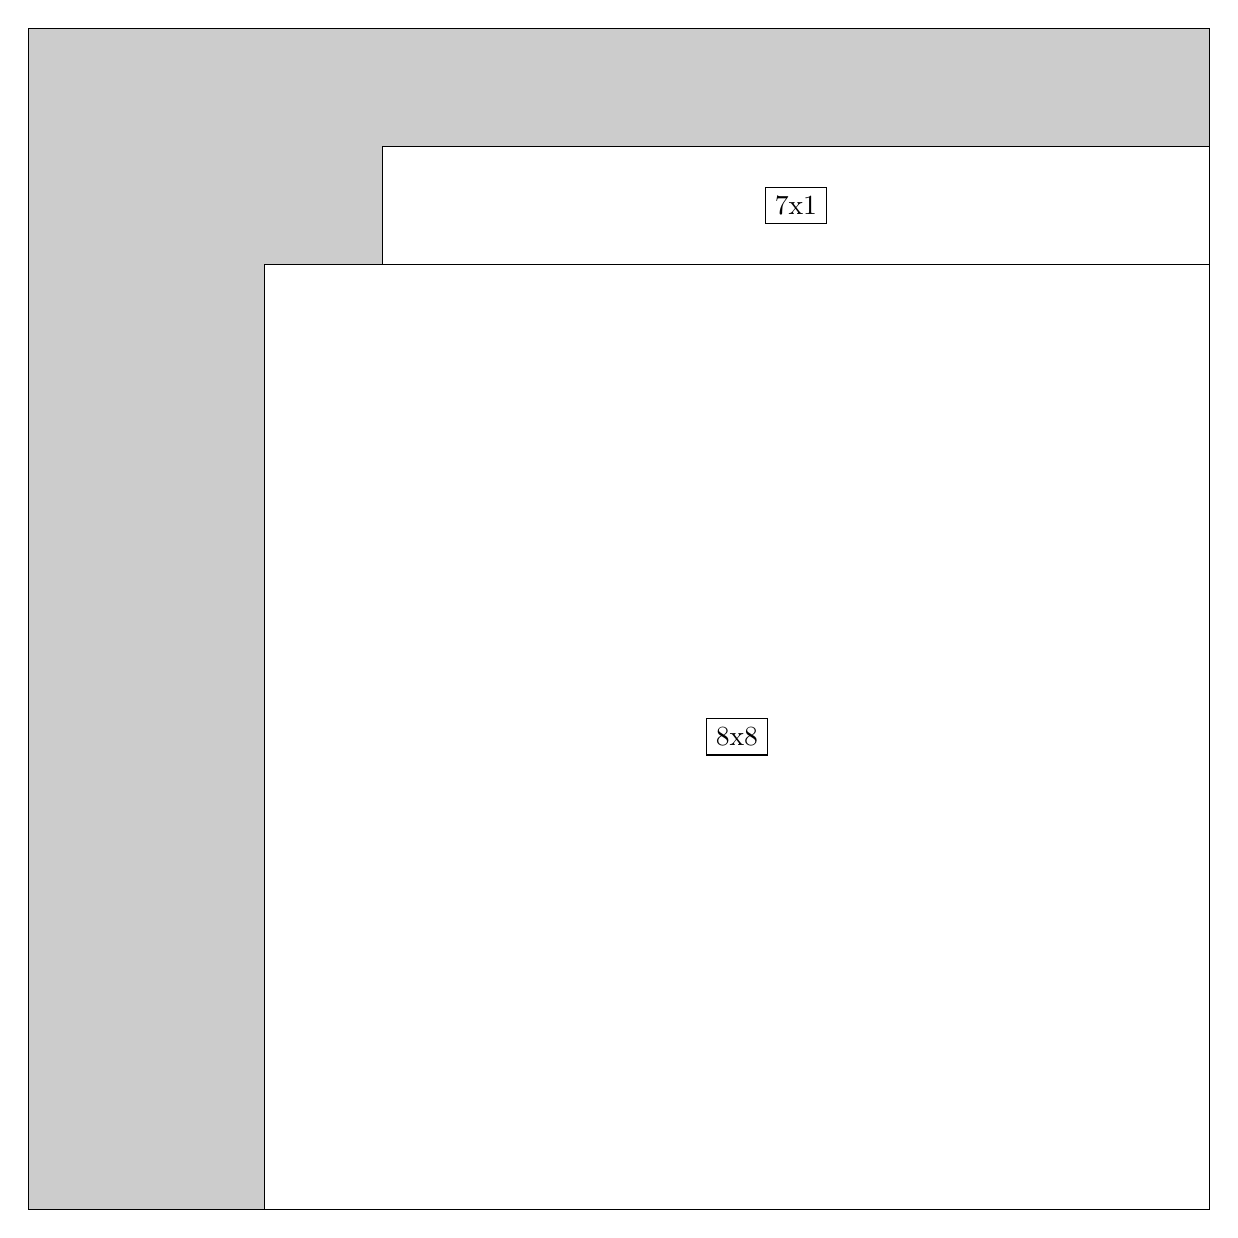
\begin{tikzpicture}[shorten >=1pt,scale=1.0,every node/.style={scale=1.0},->]
\tikzstyle{vertex}=[circle,fill=black!25,minimum size=14pt,inner sep=0pt]
\filldraw[fill=gray!40!white, draw=black] (0,0) rectangle (15.0,15.0);
\foreach \name/\x/\y/\w/\h in {8x8/3.0/0.0/12.0/12.0,7x1/4.5/12.0/10.5/1.5}
\filldraw[fill=white!40!white, draw=black] (\x,\y) rectangle node[draw] (\name) {\name} ++(\w,\h);
\end{tikzpicture}


w =8 , h =8 , x =2 , y =0 , v =64
\par
w =7 , h =1 , x =3 , y =8 , v =7
\par
\newpage


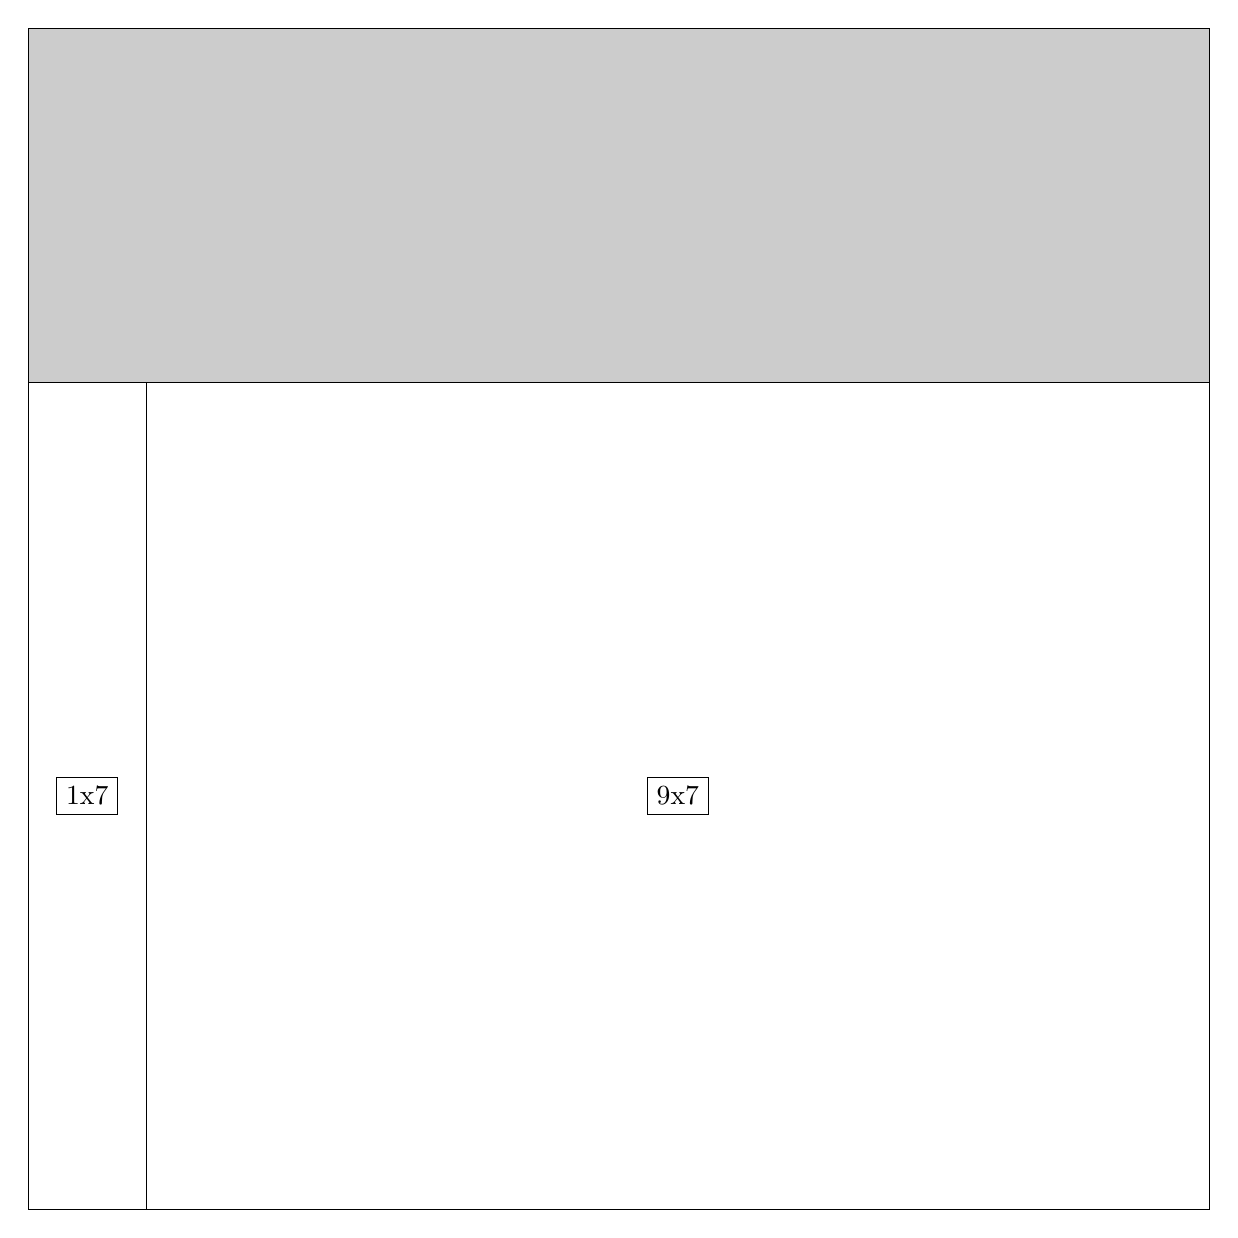
\begin{tikzpicture}[shorten >=1pt,scale=1.0,every node/.style={scale=1.0},->]
\tikzstyle{vertex}=[circle,fill=black!25,minimum size=14pt,inner sep=0pt]
\filldraw[fill=gray!40!white, draw=black] (0,0) rectangle (15.0,15.0);
\foreach \name/\x/\y/\w/\h in {9x7/1.5/0.0/13.5/10.5,1x7/0.0/0.0/1.5/10.5}
\filldraw[fill=white!40!white, draw=black] (\x,\y) rectangle node[draw] (\name) {\name} ++(\w,\h);
\end{tikzpicture}


w =9 , h =7 , x =1 , y =0 , v =63
\par
w =1 , h =7 , x =0 , y =0 , v =7
\par
\newpage


\begin{tikzpicture}[shorten >=1pt,scale=1.0,every node/.style={scale=1.0},->]
\tikzstyle{vertex}=[circle,fill=black!25,minimum size=14pt,inner sep=0pt]
\filldraw[fill=gray!40!white, draw=black] (0,0) rectangle (15.0,15.0);
\foreach \name/\x/\y/\w/\h in {7x6/4.5/0.0/10.5/9.0,3x6/0.0/0.0/4.5/9.0,10x4/0.0/9.0/15.0/6.0}
\filldraw[fill=white!40!white, draw=black] (\x,\y) rectangle node[draw] (\name) {\name} ++(\w,\h);
\end{tikzpicture}


w =7 , h =6 , x =3 , y =0 , v =42
\par
w =3 , h =6 , x =0 , y =0 , v =18
\par
w =10 , h =4 , x =0 , y =6 , v =40
\par
\newpage


\begin{tikzpicture}[shorten >=1pt,scale=1.0,every node/.style={scale=1.0},->]
\tikzstyle{vertex}=[circle,fill=black!25,minimum size=14pt,inner sep=0pt]
\filldraw[fill=gray!40!white, draw=black] (0,0) rectangle (15.0,15.0);
\foreach \name/\x/\y/\w/\h in {8x10/3.0/0.0/12.0/15.0,1x10/1.5/0.0/1.5/15.0,1x10/0.0/0.0/1.5/15.0}
\filldraw[fill=white!40!white, draw=black] (\x,\y) rectangle node[draw] (\name) {\name} ++(\w,\h);
\end{tikzpicture}


w =8 , h =10 , x =2 , y =0 , v =80
\par
w =1 , h =10 , x =1 , y =0 , v =10
\par
w =1 , h =10 , x =0 , y =0 , v =10
\par
\newpage


\end{document}